% วัดก่อนเชื่อ — Thai edition of main.tex (full translation + glossary appendix)
% Same structure, labels and claim tags ([Cnn] in %-comments) as main.tex, so the audit can pair
% the two editions. Arabic numerals only (no Thai digits). Thai line breaking: XeTeX + ICU
% dictionary segmentation via \XeTeXlinebreaklocale "th". Font: Sarabun (SIL OFL 1.1, fonts/sarabun/).
% Build: tectonic main_th.tex
\documentclass[11pt,a4paper]{article}
\usepackage[margin=2.4cm]{geometry}
\usepackage{fontspec}
\usepackage{amsmath}
\usepackage{graphicx}
\usepackage{booktabs}
\usepackage{longtable}
\usepackage{array}
\usepackage{xcolor}
\usepackage{etoolbox}
\usepackage[font=small,labelfont=bf,justification=raggedright,singlelinecheck=false]{caption}
\usepackage[numbers,sort&compress]{natbib}
\usepackage[hidelinks]{hyperref}
\usepackage{enumitem}
\usepackage{placeins}
\setlist{itemsep=2pt,topsep=4pt}
\setlength{\parskip}{3pt}
\renewcommand{\arraystretch}{1.12}
\newcommand{\R}{\ensuremath{R}}

% ── Thai typesetting ─────────────────────────────────────────────────────────
\setmainfont{Sarabun}[Path=fonts/sarabun/, Extension=.ttf, UprightFont=*-Regular,
  BoldFont=*-Bold, ItalicFont=*-Italic, BoldItalicFont=*-BoldItalic]
\XeTeXlinebreaklocale "th"            % ICU dictionary-based Thai word segmentation
\XeTeXlinebreakskip = 0pt             % zero-width break opportunity between Thai words (no stretch:
                                       % justified Thai shows visible gaps inside phrases)
\usepackage{ragged2e}
\AtBeginDocument{\RaggedRight}         % ragged-right, as in normal Thai body text
\setlength{\RaggedRightParindent}{1.5em}
\hyphenpenalty=10000                   % no English-style hyphenation of Latin words (e.g. XAUUSD)
\emergencystretch=2em
\linespread{1.12}                      % room for Thai stacked vowels and tone marks
% \tw{...}: a word that ICU's dictionary mis-segments (mostly transliterated loanwords).
% The word itself cannot break; zero-width glue on both sides keeps a break opportunity
% before and after it.
% The word list lives in tools/th_protected_words.txt; tools/th_protect.py applies it.
\newcommand{\tw}[1]{\texorpdfstring{\hspace{0pt}\mbox{#1}\hspace{0pt}}{#1}}
\renewcommand{\figurename}{ภาพที่}
\renewcommand{\tablename}{ตารางที่}
\renewcommand{\abstractname}{บทคัดย่อ}
\renewcommand{\refname}{เอกสารอ้างอิง}
\renewcommand{\appendixname}{ภาคผนวก}
% Sarabun has no small caps: the English evidence labels (Falsified, Not supported, ...) are set in
% small uppercase instead, as in the figures.
\renewcommand{\textsc}[1]{{\small\MakeUppercase{#1}}}

% generated by paper/tools/captions_to_tex.py from figures/captions_th.md -- do not edit
\csdef{capth-F1}{การปรับเทียบระบบทดสอบบนข้อมูลชุดเดียวกัน (แท่ง M5 จำนวน 165,437 แท่ง) และโค้ดกลยุทธ์ชุดเดียวกัน การรันทั้งสองต่างกันเฉพาะกฎการตัดหน้าต่างข้อมูล (a) แท่งที่แรเงาเป็นเส้นทแยงคือสถิติต่อขาแบบเดิม การเปลี่ยนเป็นหน่วยต่อสัญญาณ แล้วจึงเปลี่ยนเป็นการตัดหน้าต่างตามเวลาปิดของแท่ง ทำให้ค่า t ลดลงจาก +3.345 เป็น +2.453 และเป็น +0.917 (b) \tw{ค่าคาดหมาย}ต่อสัญญาณ พร้อมช่วงความเชื่อมั่น 95\% ที่คำนวณกลับจากค่า t ที่รายงาน (SE = mean/t) การตั้งค่าแบบจับคู่\tw{คำสั่ง}ด้วย limit order และคิดต้นทุนการ\tw{ซื้อขาย} \emph{ที่มา:} \texttt{report\_calib\_v1\_full.json} (SHA-256 \texttt{611cf0bbc7003970}\ldots{}); \texttt{report\_calib\_v2\_full.json} (SHA-256 \texttt{c71ed4c181c1f610}\ldots{}).}
\csdef{capth-F2}{ผลตอบแทนสะสม (บน) และการลดลงจากจุดสูงสุดก่อนหน้า (ล่าง) ของการรันปรับเทียบทั้งสองใน\tw{ภาพที่}~\ref{fig:F1} คิดเป็นร้อยละของเงินทุนเริ่มต้นจำลอง โดยเก็บค่าที่แท่งสุดท้ายของแต่ละวัน การเก็บค่ารายวันทำให้ค่าที่แสดง\tw{ต่ำกว่า}การลดลงสูงสุดภายในแท่งที่ระบบทดสอบรายงาน (ระบบเดิม 4.82\%, harness-v2 5.43\%) ภายใต้ระบบที่แก้ไขแล้ว ผลตอบแทนลดลง แต่การลดลงสูงสุดไม่ได้ลดลงตาม \emph{ที่มา:} \texttt{report\_calib\_v1\_full.json} (SHA-256 \texttt{611cf0bbc7003970}\ldots{}); \texttt{report\_calib\_v2\_full.json} (SHA-256 \texttt{c71ed4c181c1f610}\ldots{}).}
\csdef{capth-F3}{สัดส่วนของจุด\tw{ตัดสินใจ}บนแท่ง M5 ที่สุ่มมา 1000 จุด ซึ่งหน้าต่างข้อมูล H1 ณ จุดนั้นมีแท่งราคาที่ยังไม่ปิด วิธีตัดหน้าต่างแบบเดิม: 915/1000; อัตราตามทฤษฎีสำหรับจุด\tw{ตัดสินใจ} M5 ภายในหนึ่งชั่วโมง: 55/60; harness-v2: 0/1000 (การทดสอบบังคับ ใช้ seed คงที่ รันซ้ำเมื่อ 2026-11-01) \emph{ที่มา:} \texttt{paper/\allowbreak{}figures/\allowbreak{}data/\allowbreak{}test\_no\_lookahead\_run\_2026-11-01.txt} (SHA-256 \texttt{8665c4f57915bc68}\ldots{}); \texttt{tests/\allowbreak{}test\_no\_lookahead.py} (SHA-256 \texttt{875305ae0c521f07}\ldots{}).}
\csdef{capth-F4}{กลยุทธ์โซนอุปสงค์--อุปทานแบบลงทะเบียน\tw{ล่วงหน้า}บนชุดข้อมูล DEV (2024) T1 คือข้อกำหนดที่ตรึงไว้ T2--T4 เปลี่ยนพารามิเตอร์คุณภาพของโซนสองตัว (การรันทั้งสี่ครั้งคือแถวที่ 1--4 ของสมุดบันทึกการทดลองแบบเพิ่มได้อย่างเดียว) จุดคือ\tw{ค่าคาดหมาย}ต่อสัญญาณหลังหักต้นทุน แถบคือช่วง 95\% ที่คำนวณกลับจากค่า t ที่รายงาน (SE = mean/t) เส้นประคือเกณฑ์ที่ลงทะเบียนไว้\tw{ล่วงหน้า} T1 t = $-$2.793 ค่าประมาณทุกจุดติดลบ และทุกช่วงอยู่\tw{ต่ำกว่า}เกณฑ์ \emph{ที่มา:} \texttt{report\_zone\_dev\_t1.json} (SHA-256 \texttt{8e78f735b0f4b135}\ldots{}); \texttt{report\_zone\_dev\_t2.json} (SHA-256 \texttt{680cfa7bc39d4ac3}\ldots{}); \texttt{report\_zone\_dev\_t3.json} (SHA-256 \texttt{cabb08e7febc8bc5}\ldots{}); \texttt{report\_zone\_dev\_t4.json} (SHA-256 \texttt{3b6de201b05e0ac0}\ldots{}); \texttt{trials.csv} (SHA-256 \texttt{8334fec3d4328530}\ldots{}); \texttt{specs/\allowbreak{}phase1\_zone\_spec\_v1.md} (SHA-256 \texttt{03ddb7b216a925c0}\ldots{}).}
\csdef{capth-F5}{ลำดับการคัดกรองสัญญาณของข้อกำหนดโซนที่ตรึงไว้บนชุด DEV การแตะที่ไม่ได้เข้า\tw{ซื้อขาย}: 74 ครั้งถูกข้ามเพราะกฎเปิดสถานะได้ครั้งละหนึ่งสถานะ และ 28 ครั้งถูกข้ามเพราะกฎราคาเปิดกระโดดข้ามจุดตัดขาดทุน \emph{ที่มา:} \texttt{report\_zone\_dev\_t1.json} (SHA-256 \texttt{8e78f735b0f4b135}\ldots{}).}
\csdef{capth-F6}{\tw{แนวคิดที่}มีเอกสารยืนยัน 15 แนวคิดและป้ายระบุระดับ\tw{หลักฐาน} (\tw{ตารางที่}~\ref{tab:ideas}) ช่องที่มีเครื่องหมาย † (ขอบเส้นประ) อิงบันทึกที่ลงวันที่ไว้ในขณะนั้น ซึ่งไม่ได้รัน\tw{สคริปต์}ที่สร้างผลซ้ำ (ระดับ B) \textsuperscript{1}พบ\tw{ส่วนชดเชย}ความเสี่ยง แต่ความเสี่ยงส่วนหางไม่สอดคล้องกับเพดานการลดลงของมูลค่า 10\% \textsuperscript{2}ผ่านเกณฑ์ระยะที่ 1 แต่ไม่มีผลตอบแทนส่วนเกิน (alpha) ที่มีนัยสำคัญเหนือกองทุน ETF ประเภท managed futures ที่ซื้อได้ทั่วไป 'Not supported' หมายถึงไม่พบ\tw{หลักฐาน}ของความได้เปรียบ ไม่ใช่\tw{หลักฐาน}ว่าไม่มีความได้เปรียบ แหล่งที่มาของแต่ละแนวคิดระบุตามรหัส\tw{ข้อกล่าวอ้าง}ในตาราง\tw{ข้อกล่าวอ้าง} \emph{ที่มา:} \texttt{paper/\allowbreak{}claims.csv} (SHA-256 \texttt{3deb8b61a7ee262f}\ldots{}).}
\csdef{capth-F7}{เหตุใดการวัดซ้ำจึงเป็น\tw{หลักฐาน}ที่อ่อน ค่า t ต่อสัญญาณของกลุ่มย่อย SMC ที่มี timing flag $\geq$2: ในตัวอย่าง (กลุ่มย่อยถูกเลือกหลังเห็นข้อมูลชุดนี้) t = +3.045, n = 228; หน้าต่างที่รันซ้ำ t = +0.06, n = 37 หน้าต่างที่รันซ้ำอยู่ภายในช่วงข้อมูลในตัวอย่าง จึงไม่ใช่การทดสอบนอกตัวอย่าง แถบแสดงค่า t ที่คาดไว้ที่แต่ละ n หากอัตราส่วน\tw{ชาร์ป}ต่อสัญญาณในตัวอย่าง (0.202) เป็นค่าจริง ผลการวัดซ้ำอยู่ภายในแถบนั้น ทั้งสองฝั่งรันบนระบบทดสอบแบบเดิม \emph{ที่มา:} \texttt{report\_full.json} (SHA-256 \texttt{a7fedee66dc7badc}\ldots{}); \texttt{report\_w1.json} (SHA-256 \texttt{8c76ed83a99772f3}\ldots{}); \texttt{report\_w2.json} (SHA-256 \texttt{476833c1c1aa009c}\ldots{}); \texttt{report\_w3.json} (SHA-256 \texttt{cd33449fc8eec236}\ldots{}); \texttt{report\_w4.json} (SHA-256 \texttt{a849526720e1a6c8}\ldots{}); \texttt{report\_w5.json} (SHA-256 \texttt{ecfc8198f9d91cf1}\ldots{}).}
\csdef{capth-F8}{สถาปัตยกรรมของระบบขณะทำงาน วาดจาก\tw{คำสั่ง} publish/subscribe ที่มีอยู่จริงในโค้ด (ชื่อหัวข้อของ event bus แสดงด้วยตัวอักษรความกว้างคงที่) เส้นทางการหยุดระบบทั้งสองทาง ได้แก่ ข้อมูลไม่ตรงกันจากการ\tw{กระทบยอด}ใน trade logger และการจับคู่\tw{คำสั่ง} (fill) ที่ยืนยันไม่ได้ใน order executor จะส่งสัญญาณ SYSTEM\_SHUTDOWN ซึ่งหยุดการ\tw{ซื้อขาย}โดยไม่ปิดสถานะที่ถืออยู่ เส้นทางการ\tw{ตัดสินใจ}ตั้งแต่ข้อมูลแท่งราคาจนถึง\tw{คำสั่ง}\tw{ซื้อขาย}เป็นแบบกำหนดแน่นอน (deterministic) ส่วนประกอบโมเดลภาษาซึ่งเป็นทางเลือกทำหน้าที่เพียงให้\tw{คำแนะนำ}รายชั่วโมงบนกรอบเวลาที่ใหญ่กว่า และปิดไว้เป็นค่าเริ่มต้น ส่วนประกอบรอง (ตัวติดตามจุดคุ้มทุน ตัวจัดการ\tw{คำสั่ง}รอ ตัวแจ้งเตือน ตัวส่งออกสถานะ ตัวติดตามระบบ และตัวปิดสถานะฉุกเฉิน) ถูกละไว้เพื่อให้อ่านง่าย \emph{ที่มา:} \texttt{main.py} (SHA-256 \texttt{a01eb656a6ec7efd}\ldots{}); \texttt{core/\allowbreak{}event\_bus.py} (SHA-256 \texttt{9d08645d45403b69}\ldots{}); \texttt{agents/\allowbreak{}risk\_manager.py} (SHA-256 \texttt{1dfa09df59084abe}\ldots{}); \texttt{execution/\allowbreak{}order\_executor.py} (SHA-256 \texttt{f3fdfe9f9b680891}\ldots{}); \texttt{memory/\allowbreak{}trade\_logger.py} (SHA-256 \texttt{1688bb607d715397}\ldots{}).}
\csdef{capth-F9}{ลำดับเหตุการณ์ในการศึกษากลยุทธ์โซน จากเวลาที่บันทึกใน git commit และเวลาที่บันทึกในสมุดบันทึกการทดลองเอง (เวลา UTC; ด้านซ้ายแสดงช่วงห่างระหว่างเหตุการณ์ที่ต่อเนื่องกัน) ข้อกำหนดของกลยุทธ์ (\tw{ความน่าจะเป็น}\tw{ล่วงหน้า} เกณฑ์ G2 และการแบ่งชุดข้อมูล) ถูก commit ก่อนที่จะมีการบันทึกแถวแรกของสมุดบันทึก 21.4 ชั่วโมง เวลาในสมุดบันทึกเป็นเวลาที่การรันเสร็จสิ้น โดยไม่มีการบันทึกเวลาเริ่ม การรัน\tw{ครั้งแรก}จึงอาจเริ่มขึ้นก่อน commit ของ engine เพียง\tw{เล็กน้อย} \tw{ภาคผนวก}ที่มาของพารามิเตอร์ในข้อกำหนดระบุว่าไม่มีการคำนวณค่าสถิติใด ๆ บนชุดข้อมูลส่วนใดเลยก่อนการตรึงข้อกำหนด การแก้ไขข้อกำหนดเพียงครั้งเดียวหลังจากนั้นคือ\tw{ภาคผนวก}ดังกล่าว (เพิ่ม 40 บรรทัด ลบ 0 บรรทัด) แถวที่ 2--4 ถูกเลือกหลังแถวที่ 1 ภายใต้ข้อกำหนดที่อนุญาตให้ปรับแต่งบนชุด DEV ได้ เวลา commit บันทึกโดยเครื่องของผู้เขียนเอง และไม่\tw{ได้รับ}การรับรองจากบุคคลภายนอก \emph{ที่มา:} \texttt{paper/\allowbreak{}figures/\allowbreak{}data/\allowbreak{}git\_timeline\_utc.txt} (SHA-256 \texttt{94bca4ed34c7db10}\ldots{}); \texttt{trials.csv} (SHA-256 \texttt{8334fec3d4328530}\ldots{}); \texttt{specs/\allowbreak{}phase1\_zone\_spec\_v1.md} (SHA-256 \texttt{03ddb7b216a925c0}\ldots{}); \texttt{paper/\allowbreak{}figures/\allowbreak{}data/\allowbreak{}spec\_appendix\_numstat\_8634f34.txt} (SHA-256 \texttt{4f2bfe6ee91d7c32}\ldots{}).}


\title{วัดก่อนเชื่อ:\\[2pt]
\large การศึกษาเชิงหักล้างสมมติฐานแบบลงทะเบียนล่วงหน้า\\ของกลยุทธ์โครงสร้างราคาสำหรับนักลงทุนรายย่อยบน XAUUSD\\[4pt]
\normalsize\emph{Measuring Before Believing: A Pre-Registered Falsification Study of Retail
Price-Structure Strategies on XAUUSD}}
\author{SuperKICKY01\\\small นักวิจัยอิสระระดับนักเรียน ประเทศไทย\\\small รายงานทางเทคนิคอิสระ ---
ยังไม่ผ่านการประเมินโดยผู้ทรงคุณวุฒิ (peer review)}
\date{พฤศจิกายน ค.ศ. 2026 (พ.ศ. 2569) \quad (ฉบับภาษาไทย แปลจากฉบับภาษาอังกฤษ)}

\begin{document}
\maketitle

\begin{abstract}
\noindent
การสอนการ\tw{ซื้อขาย}สำหรับนักลงทุน\tw{รายย่อย}มักเผยแพร่กฎการเข้า\tw{ซื้อขาย}ที่อิงกับโครงสร้างราคาที่มองเห็นได้
เช่น \tw{ออร์เดอร์บล็อก} (order block) และโซนอุปสงค์--อุปทาน (supply/demand zone)
รายงานฉบับนี้ตั้งคำถามว่า กฎสองกลุ่มดังกล่าวแสดงความได้เปรียบ (edge) ต่อสัญญาณที่วัดได้บนข้อมูล
XAUUSD ราย 5 นาทีหรือไม่ เมื่อการทดสอบย้อนหลัง (backtest) ใช้เฉพาะข้อมูลที่มีอยู่จริง ณ เวลา\tw{ตัดสินใจ}
(causal) และการอนุมานทางสถิติใช้หน่วยที่เป็นอิสระต่อกัน ผู้วิจัยพบข้อบกพร่องสองประการในระบบทดสอบย้อนหลังเดิมของโครงการเอง
ได้แก่ หน้าต่างข้อมูลกรอบเวลาใหญ่มีแท่งราคาที่ยังไม่ปิดอยู่ใน 91.5\% ของจุด\tw{ตัดสินใจ}
และนัยสำคัญทางสถิติถูกคำนวณต่อขาของสถานะ (position leg) แทนที่จะคำนวณต่อสัญญาณ
เมื่อแก้ไขทั้งสองประการบนข้อมูลและโค้ดชุดเดียวกัน ค่าสถิติ $t$ ต่อสัญญาณของกลยุทธ์\tw{ออร์เดอร์บล็อก}ลดลงจาก
$+2.45$ เหลือ $+0.92$ ($n=77$) จากนั้นผู้วิจัยได้กำหนดกลยุทธ์โซนอุปสงค์--อุปทาน
และ commit ข้อกำหนดก่อนที่จะมีผลการทดสอบย้อนหลัง\tw{ครั้งแรก} แล้วทดสอบบนชุดข้อมูลสำหรับการพัฒนาเท่านั้น
ผลที่ได้คือ\tw{ค่าคาดหมาย}ต่อสัญญาณ $-0.143\R$ และ $t=-2.79$ ($n=406$)
เทียบกับเกณฑ์ที่ลงทะเบียนไว้\tw{ล่วงหน้า}ว่าต้องได้\tw{อย่างน้อย} $+0.15\R$
การรันเพิ่มเติมอีกสามครั้งซึ่งเลือกหลังจากการรัน\tw{ครั้งแรก}ก็ให้\tw{ค่าคาดหมาย}ติดลบเช่นกัน
ชุดข้อมูลสำหรับการประเมินผลไม่ได้ถูกใช้ รายงานนี้นำเสนอ\tw{แนวคิดที่}มีเอกสารยืนยัน 15 แนวคิด
พร้อมป้ายระบุระดับ\tw{หลักฐาน}อย่างชัดเจน และแก้ไขข้อผิดพลาดสามประการในเอกสารก่อนหน้าของโครงการ
สิ่งที่รายงานนี้มีส่วนร่วมคือกรณีศึกษาที่มีเอกสารครบถ้วนและ\tw{เครื่องมือ}\tw{ตรวจสอบ}ความถูกต้องที่เปิดเผยต่อสาธารณะ
มิใช่วิธีการใหม่
\end{abstract}

% ════════════════════════════════════════════════════════════════════════════
\section{บทนำ}

กลยุทธ์ที่สร้างขึ้นบนพื้นฐานของ ``โครงสร้างราคา'' (price structure) เช่น \tw{ออร์เดอร์บล็อก}
การทะลุโครงสร้าง (break of structure) และโซนอุปสงค์--อุปทาน
\tw{ได้รับ}การสอนอย่างแพร่หลายแก่นักลงทุน\tw{รายย่อย} หลักคิดของกลยุทธ์เหล่านี้คือ
ราคาจะกลับมาที่ระดับซึ่งมี\tw{คำสั่ง}\tw{ซื้อขาย}กระจุกตัวอยู่ และผู้ที่เข้า\tw{ซื้อขาย}เมื่อราคากลับมาจะ\tw{ได้รับ}ผลตอบแทนจากการทำเช่นนั้น
\tw{หลักฐาน}เกี่ยวกับการเก็งกำไรของนักลงทุน\tw{รายย่อย}ไม่น่าพอใจนัก
กล่าวคือ นักลงทุนรายบุคคลโดยรวมขาดทุนจากการ\tw{ซื้อขาย} \citep{barber2009lose}
และในกลุ่มผู้\tw{ซื้อขาย}ระหว่างวัน (day trader) มีเพียงส่วนน้อยที่แสดงความสามารถในการทำกำไรได้อย่างต่อเนื่อง
\citep{barber2014daytrading} อย่างไรก็ตาม คำถามว่ากฎของนักลงทุน\tw{รายย่อย}กฎใดกฎหนึ่งมีความได้เปรียบหรือไม่
เป็นคำถามเชิงประจักษ์ ซึ่งการทดสอบย้อนหลังที่รัดกุมสามารถตอบได้ด้วยต้นทุนต่ำ

รายงานฉบับนี้บันทึกความพยายามครั้งหนึ่งในการตอบคำถามดังกล่าวสำหรับ XAUUSD
(ทองคำในตลาดทันทีเทียบกับดอลลาร์สหรัฐ) บนแท่งราคาราย 5 นาที
และโดยเฉพาะอย่างยิ่ง บันทึกว่าต้องทำสิ่งใดบ้างก่อนที่คำตอบจะเชื่อถือได้ คำถามวิจัยคือ

\begin{quote}
\emph{กฎโครงสร้างราคาของนักลงทุน\tw{รายย่อย}สองกลุ่ม---กฎการประกอบกันของ\tw{ออร์เดอร์บล็อก}
(order-block confluence) และกฎโซนอุปสงค์--อุปทาน---แสดงความได้เปรียบต่อสัญญาณที่วัดได้บนข้อมูล
XAUUSD M5 หรือไม่ เมื่อการทดสอบย้อนหลังใช้เฉพาะข้อมูลที่มีอยู่จริง ณ เวลา\tw{ตัดสินใจ}
และการอนุมานทางสถิติทำบนหน่วยที่เป็นอิสระต่อกัน}
\end{quote}

สิ่งที่รายงานนี้มีส่วนร่วมมีขอบเขตจำกัด และขอระบุตามนั้น ดังนี้
\begin{enumerate}
\item กรณีตัวอย่างที่แสดงให้เห็นว่าข้อบกพร่องสองประการในระบบทดสอบย้อนหลัง (backtest harness)
ทำให้ความได้เปรียบที่ปรากฏสูงเกินจริงได้อย่างไร โดยวัดปริมาณบนข้อมูลและโค้ดกลยุทธ์ชุดเดียวกัน
(\tw{ส่วนที่}~\ref{sec:res-g0})
\item การทดสอบเพื่อหักล้างสมมติฐาน (falsification) ของกลยุทธ์โซนอุปสงค์--อุปทาน
แบบลงทะเบียน\tw{ล่วงหน้า} พร้อมสมุดบันทึกการทดลองที่เพิ่มได้อย่างเดียว (append-only trial ledger)
ซึ่งหยุดที่ขั้นการพัฒนา เพื่อให้ข้อมูลสำหรับการประเมินผลยังคงไม่ถูกใช้ (\tw{ส่วนที่}~\ref{sec:res-zone})
\item ทะเบียน\tw{แนวคิดที่}มีเอกสารยืนยัน 15 แนวคิด พร้อมป้ายระบุระดับ\tw{หลักฐาน}และชั้นของ\tw{หลักฐาน}
รวมถึง\tw{แนวคิดที่}ยังไม่ได้ทดสอบ (\tw{ส่วนที่}~\ref{sec:res-register})
\item ตัว\tw{เครื่องมือ}\tw{ตรวจสอบ}ความถูกต้องเอง ได้แก่ การตัดหน้าต่างข้อมูลตามเวลาปิดของแท่งพร้อมการทดสอบบังคับ
สถิติต่อสัญญาณ และสมุดบันทึกการทดลอง ซึ่งเผยแพร่พร้อมค่าแฮชของไฟล์\tw{หลักฐาน}ทุกไฟล์
(\tw{ภาคผนวก}~\ref{app:repro})
\end{enumerate}
รายงานนี้ไม่ได้เสนอวิธีการทางสถิติใหม่ และไม่ได้อ้างว่าโครงสร้างราคาไม่สามารถมีข้อมูลที่เป็นประโยชน์ได้โดยทั่วไป
ข้อความว่า ``ไม่พบ\tw{หลักฐาน}ของความได้เปรียบ'' ไม่ใช่ข้อความเดียวกับ ``ไม่มีความได้เปรียบ''

% ════════════════════════════════════════════════════════════════════════════
\section{งานวิจัยที่เกี่ยวข้อง}

\paragraph{การปรับแต่งเกินพอดีในการทดสอบย้อนหลังและอคติจากการคัดเลือก}
เมื่อทดลองการตั้งค่าหลายแบบแล้วรายงานเฉพาะแบบที่ดีที่สุด อัตราส่วน\tw{ชาร์ป} (Sharpe ratio)
ของแบบนั้นจะเอนเอียงสูงเกินจริง อัตราส่วน\tw{ชาร์ป}แบบปรับลด (Deflated Sharpe Ratio)
แก้ไขอัตราส่วน\tw{ชาร์ป}ที่รายงานโดยคำนึงถึงจำนวนครั้งที่ทดลองและผลตอบแทนที่ไม่ได้แจกแจงแบบปกติ
\citep{bailey2014dsr} \citet{bailey2014pseudo} เสนอว่าการปรับแต่งเกินพอดีในการทดสอบย้อนหลัง
(backtest overfitting) เป็นเหตุผลที่เป็นไปได้ว่าทำไมกลยุทธ์ที่ดูทำกำไรในการทดสอบย้อนหลัง
จึงล้มเหลวกับข้อมูลนอกตัวอย่าง (out of sample) และ \citet{bailey2017pbo}
เสนอวิธีการ\tw{ตรวจสอบ}ไขว้แบบสมมาตรเชิงการจัดหมู่ (combinatorially symmetric cross-validation)
เพื่อประมาณ\tw{ความน่าจะเป็น}ที่การตั้งค่าที่ถูกเลือกเป็นผลจากการปรับแต่งเกินพอดี
การ\tw{ตรวจสอบ}ไขว้แบบตัดข้อมูล\tw{ทับซ้อน} (purged cross-validation) สำหรับอนุกรมเวลาทางการเงิน
อธิบายไว้โดย \citet{lopezdeprado2018afml}

\paragraph{การทดสอบหลายสมมติฐานพร้อมกันในการเงิน}
\citet{harvey2016cross} มองตัวแปรพยากรณ์ผลตอบแทนจำนวนมากที่มีผู้อ้างไว้ในวรรณกรรม
ว่าเป็นปัญหาการทดสอบหลายสมมติฐานพร้อมกัน (multiple testing) และเสนอว่าปัจจัยใหม่ควรผ่านค่าสถิติ
$t$ ประมาณ 3.0 แทนที่จะเป็น 2.0 การควบคุมอัตราการ\tw{ค้นพบ}เท็จ (false discovery rate)
\citep{benjamini1995fdr} เป็นทางเลือกมาตรฐานแทนการควบคุมความ\tw{คลาดเคลื่อน}รวมของทั้งกลุ่ม
(family-wise error) เมื่อต้องคัดกรองสมมติฐานจำนวนมาก
และถูกใช้ในแนวคิดหนึ่งใน\tw{ส่วนที่}~\ref{sec:res-register}

\paragraph{ผลการดำเนินงานของนักลงทุน\tw{รายย่อย}}
จากบันทึกการ\tw{ซื้อขาย}ฉบับสมบูรณ์ของไต้หวัน \citet{barber2009lose}
พบว่าการ\tw{ซื้อขาย}ของนักลงทุนรายบุคคลก่อให้เกิดผลขาดทุนอย่างเป็นระบบในปริมาณมาก และ
\citet{barber2014daytrading} พบว่าแม้จะมีผู้\tw{ซื้อขาย}ระหว่างวันกลุ่มเล็ก ๆ
ที่ได้ผลตอบแทนเป็นบวกอย่างคาดการณ์ได้ แต่\tw{ภาพรวม}ของทั้งกลุ่มถูกครอบงำด้วยผลขาดทุน

\paragraph{การกระจุกตัวของ\tw{คำสั่ง}\tw{ซื้อขาย}ที่ระดับราคา}
\tw{หลักฐาน}จากฝั่งสถาบันที่ใกล้เคียงที่สุดว่าทำไมระดับราคาจึงอาจมีความสำคัญ
มาจากข้อมูล\tw{คำสั่ง}\tw{ซื้อขาย}ในตลาดอัตราแลกเปลี่ยน \citet{osler2003currency}
บันทึกว่า\tw{คำสั่ง}ทำกำไร (take-profit) กระจุกตัวที่ตัวเลขกลม และ\tw{คำสั่ง}ตัดขาดทุน (stop-loss)
กระจุกตัวเลยตัวเลขเหล่านั้นไป\tw{เล็กน้อย} และใช้ข้อเท็จจริงนี้อธิบายว่าทำไมแนวโน้มจึงมักกลับตัวที่ระดับดังกล่าว
หรือเร่งตัวเมื่อทะลุผ่าน \citet{osler2005stoploss}
พบว่าการเคลื่อนไหวของราคาที่รวดเร็วสัมพันธ์กับการทำงานของ\tw{คำสั่ง}ตัดขาดทุนที่กระจุกตัวกัน
\tw{ข้อค้นพบ}เหล่านี้เกี่ยวกับระดับราคาที่มี\tw{หลักฐาน}ว่ามี\tw{คำสั่ง}รออยู่จริง ส่วนคำถามว่าระดับที่กฎของนักลงทุน\tw{รายย่อย}ลากขึ้น
ตรงกับกลุ่ม\tw{คำสั่ง}ดังกล่าวหรือไม่นั้นเป็นอีกคำถามหนึ่ง
และการทดสอบผลตอบแทนต่อการแตะระดับแต่ละครั้งใน\tw{ส่วนที่}~\ref{sec:res-zone}
วัดผลที่ตามมาโดยตรง

\paragraph{การลงทะเบียน\tw{ล่วงหน้า}}
การกำหนดสมมติฐานและแผนการวิเคราะห์ก่อนเห็นผลลัพธ์
ช่วยแยกการพยากรณ์ (prediction) ออกจากการอธิบาย\tw{ภายหลัง} (postdiction) \citep{nosek2018prereg}
การศึกษากลยุทธ์โซนใน\tw{ส่วนที่}~\ref{sec:method-prereg} ปฏิบัติตามแนวทางนี้

\paragraph{กลยุทธ์ประเภทอื่น}
\tw{โมเมนตัม}แบบอนุกรมเวลา (time-series momentum) \citep{moskowitz2012tsmom}
และค่าความ\tw{คลาดเคลื่อน}มาตรฐานที่ทนต่อความแปรปรวนไม่คงที่และสหสัมพันธ์ในตัวเอง
(HAC standard errors; ดูอภิธานศัพท์) \citep{newey1987hac}
ปรากฏอยู่ในแนวคิดสองแนวคิดในทะเบียน

% ════════════════════════════════════════════════════════════════════════════
\section{ระบบ}
\label{sec:system}

การศึกษาทั้งหมดดำเนินการบนส่วนการทดสอบย้อนหลังของระบบ\tw{ซื้อขาย}จริงที่เขียนด้วยภาษา Python
แบบ\tw{อะซิงโครนัส} (asynchronous) สำหรับ\tw{แพลตฟอร์ม} MetaTrader~5 (MT5)
ในที่นี้จะอธิบายระบบจริงเพียงสั้น ๆ เพราะการออกแบบของระบบเป็นตัวกำหนดว่าการทดสอบย้อนหลังต้องเลียนแบบอะไร
(\tw{ภาพที่}~\ref{fig:F8})

\paragraph{สถาปัตยกรรม}
ส่วนประกอบต่าง ๆ สื่อสารกันผ่าน event bus แบบ publish/subscribe ภายใน\tw{โปรเซส}เดียวกัน
โดย \texttt{main.py} เริ่มงานหลัก 13 งาน และงานที่เป็นทางเลือกอีก 1 งาน % [C71]
การเรียกใช้\tw{เทอร์มินัล} MT5 ที่ต้องรอผล (blocking call) ทั้งหมดทำงานใน\tw{เธรด}แยก
เส้นทางตั้งแต่แท่งราคาที่เข้ามาจนถึง\tw{คำสั่ง}\tw{ซื้อขาย}เป็นแบบกำหนดแน่นอน (deterministic)
ส่วนประกอบโมเดลภาษาถูกนำออกจากเส้นทางนั้นเมื่อวันที่ 2026-06-05
และคงเหลือเพียงในฐานะที่ปรึกษารายชั่วโมงบนกรอบเวลาที่ใหญ่กว่า ซึ่งเป็นทางเลือกและปิดไว้เป็นค่าเริ่มต้น % [C62]

\paragraph{กลไกบริหารความเสี่ยง}
\tw{คำสั่ง}\tw{ซื้อขาย}ที่จะส่งทุก\tw{คำสั่ง}ต้องผ่านการยับยั้ง (veto) แบบกำหนดแน่นอนที่มีหมายเลข 9 ข้อ
และตัวตัดวงจรเมื่อขาดทุนรายวันถึงระดับที่กำหนดแบบป้องกัน\tw{ล่วงหน้า} ได้แก่ การงด\tw{ซื้อขาย}ช่วงข่าว
การขาดทุนสะสมรายวัน การขาดทุนสะสมรวม จำนวนสถานะที่เปิดพร้อมกัน ทิศทางซ้ำ
ระยะตัดขาดทุนกว้างเกินไปเมื่อเทียบกับค่าเฉลี่ยช่วงราคาจริง (average true range, ATR)
ระยะตัดขาดทุนแคบเกินไปเมื่อเทียบกับ ATR ขนาด\tw{ล็อต}เป็นศูนย์ และการ\tw{ตรวจสอบ}\tw{มาร์จิน}\tw{ล่วงหน้า} % [C57]

\paragraph{ความปลอดภัยในการส่ง\tw{คำสั่ง}}
การตอบรับจาก\tw{โบรกเกอร์}ไม่ถือว่าเป็นการจับคู่\tw{คำสั่ง}สำเร็จ (fill)
ตัวส่ง\tw{คำสั่ง} (order executor) จะรอจนกว่ารายการเปิดสถานะที่สอดคล้องกันปรากฏในประวัติรายการของ\tw{โบรกเกอร์}
ก่อนจึงจะประกาศว่าการ\tw{ซื้อขาย}สำเร็จ และจะหยุดระบบหากไม่\tw{ได้รับ}การยืนยัน % [C58, C72]
การ\tw{กระทบยอด}เป็นระยะจะเปรียบเทียบสถานะที่เปิดอยู่กับ\tw{โบรกเกอร์}กับฐานข้อมูลการ\tw{ซื้อขาย}
และหยุดระบบเมื่อพบความไม่ตรงกัน % [C59]
การหยุดระบบจะหยุดการ\tw{ซื้อขาย}ใหม่ แต่จงใจไม่ปิดสถานะที่ถืออยู่
\tw{คำสั่ง}ตัดขาดทุนและ\tw{คำสั่ง}ทำกำไรที่ฝั่ง\tw{โบรกเกอร์}ยังคงมีผลอยู่ % [C60]
การทดสอบด้วยการฉีดความผิดพลาด (fault injection) ซึ่งรวมถึงการบังคับปิด\tw{โปรเซส}ทันทีและการ\tw{ตรวจสอบ}การกู้คืน
ผ่านเกณฑ์ โดยไม่มีสถานะใดถูกบันทึกสำหรับ\tw{คำสั่ง}ที่ไม่\tw{ได้รับ}การจับคู่เลย % [C61]

\begin{figure}[htbp]
\centering
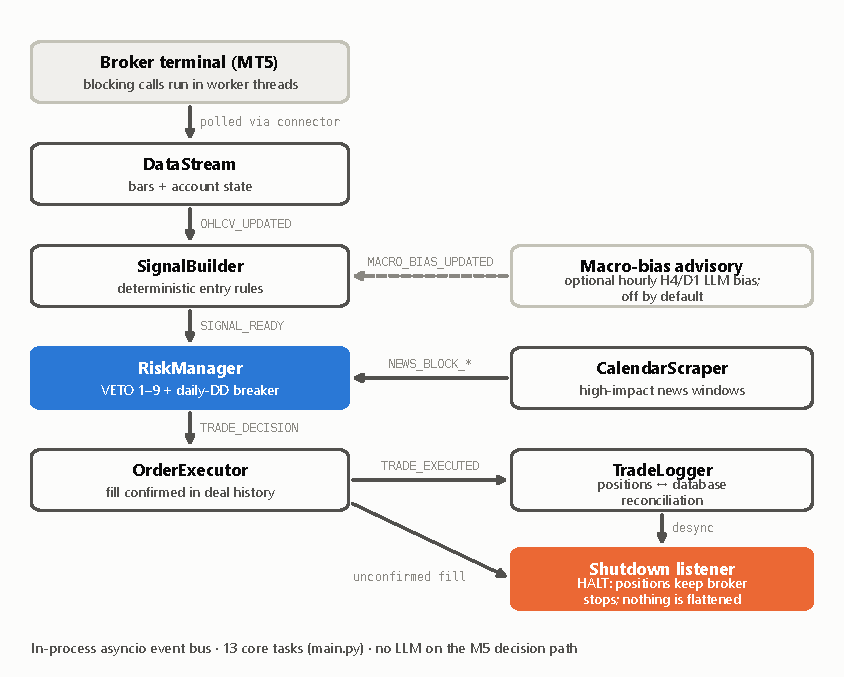
\includegraphics[width=0.82\linewidth]{figures/F8_architecture.pdf}
\caption{\csuse{capth-F8}}
\label{fig:F8}
\end{figure}

% ════════════════════════════════════════════════════════════════════════════
\section{วิธีการศึกษา}
\label{sec:method}

\subsection{ข้อมูล}
การทดสอบย้อนหลังทั้งหมดใช้ราคาเสนอซื้อ (BID) จาก Dukascopy
ซึ่งแปลงจากแท่งราย 1 นาทีเป็นแท่งราย 5 นาที จำนวน 165,437 แท่ง
ตั้งแต่ 2024-01-01 ถึง 2026-05-06 % [C14, C63]
ไฟล์ราคาไม่ได้เผยแพร่ซ้ำ (\tw{ภาคผนวก}~\ref{app:repro})
แต่เผยแพร่ค่าแฮช SHA-256 และ\tw{สคริปต์}\tw{ดาวน์โหลด} เพื่อให้สร้างไฟล์ขึ้นใหม่และ\tw{ตรวจสอบ}ได้

\subsection{การตัดหน้าต่างข้อมูลตามเวลาปิดของแท่ง (harness-v2)}
\label{sec:method-slicing}
การ\tw{ตัดสินใจ}บนแท่งราย 5 นาที (M5) ที่ปิดในเวลา $T$
ใช้ได้เฉพาะแท่งของกรอบเวลาใหญ่ที่ \emph{ปิดแล้ว} ภายในเวลา $T$ เท่านั้น
ระบบทดสอบเดิมเลือกแท่งตามป้ายเวลาเปิดของแท่ง ($\text{label}\le T$)
ซึ่งทำให้แท่งรายชั่วโมง (H1) ที่เปิดก่อน $T$ แต่ยังไม่ปิดถูกนำเข้ามาด้วย
สำหรับการ\tw{ตัดสินใจ}บน M5 ที่อยู่ภายในชั่วโมง เหตุการณ์นี้\tw{เกิดขึ้น} 11 ใน 12 จุด
และค่าสูงสุด ต่ำสุด และราคาปิดของแท่งนั้นจะทำให้ราคาในอนาคตนานสูงสุด 55 นาทีรั่วเข้าสู่การ\tw{ตัดสินใจ}
ซึ่งเรียกว่าการรั่วของข้อมูลอนาคต (lookahead bias)
ระบบที่แก้ไขแล้วจะเก็บแท่งไว้ก็ต่อเมื่อเวลาเปิดบวกความยาวของแท่งไม่เกิน $T$
การทดสอบบังคับสุ่มจุดเล่นซ้ำ 1,000 จุด และยืนยันว่าไม่มีหน้าต่างใดมีแท่งที่ปิดหลังเวลา\tw{ตัดสินใจ}
ผลคือผ่าน 1,000/1,000 และบนจุดเดียวกันนั้น กฎเดิมจะนำแท่ง H1 ที่ยังไม่ปิดเข้ามา 915 ครั้ง
(\tw{ภาพที่}~\ref{fig:F3}) % [C01–C04]

\begin{figure}[htbp]
\centering
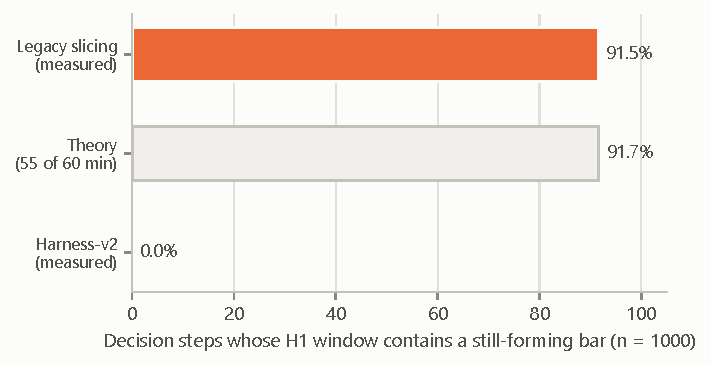
\includegraphics[width=0.66\linewidth]{figures/F3_forming_bar.pdf}
\caption{\csuse{capth-F3}}
\label{fig:F3}
\end{figure}

\subsection{สถิติต่อสัญญาณ}
\label{sec:method-persignal}
แต่ละสัญญาณเปิดสถานะสองขา (leg) ซึ่งมีระดับทำกำไรต่างกัน แต่มีจุดเข้าและจุดตัดขาดทุนเดียวกัน
ผลลัพธ์ของทั้งสองขาสัมพันธ์กันสูง การนับแต่ละขาเป็นตัวอย่างอิสระจึงทำให้นัยสำคัญสูงเกินจริงได้มากถึง
$\sqrt{2}$ เท่า หน่วยมาตรฐานของการวิเคราะห์จึงเป็นสัญญาณ
กำไรสุทธิของแต่ละสัญญาณ และผลสุทธิในหน่วย $\R$---คือจำนวนเงินที่เสี่ยงต่อสัญญาณนั้น
ซึ่งคำนวณด้วยตัวหารเดียวกับที่ใช้กำหนดขนาด\tw{ล็อต}---จะถูกรวมจากทุกขาของสัญญาณ
และค่าสถิติ $t = \bar{x}/(s/\sqrt{n})$ โดย $s$ เป็นส่วนเบี่ยงเบนมาตรฐานของตัวอย่าง
(องศาอิสระ $n-1$) % [C16]
สถิติต่อขาจะปรากฏในรายงานนี้เฉพาะเมื่ออ้างตัวเลขจากระบบเดิม และจะระบุกำกับไว้

\subsection{การลงทะเบียน\tw{ล่วงหน้า}ของการศึกษากลยุทธ์โซน}
\label{sec:method-prereg}
\begin{figure}[tbp]
\centering
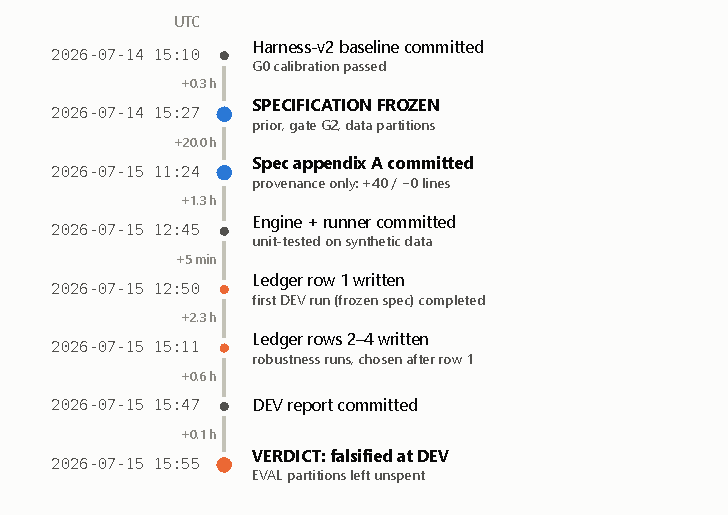
\includegraphics[width=0.54\linewidth]{figures/F9_preregistration_timeline.pdf}
\caption{\csuse{capth-F9}}
\label{fig:F9}
\end{figure}
ข้อกำหนดของกลยุทธ์โซนอุปสงค์--อุปทาน
พร้อม\tw{ความน่าจะเป็น}\tw{ล่วงหน้า} (prior) เกณฑ์ผ่าน/ไม่ผ่าน และการแบ่งชุดข้อมูล
ถูก commit เข้าระบบควบคุม\tw{เวอร์ชัน} 21.4 ชั่วโมงก่อนที่จะมีการบันทึกผลการทดสอบย้อนหลัง\tw{ครั้งแรก}
(\tw{ภาพที่}~\ref{fig:F9}) % [C68, C70]
\begin{itemize}
\item \textbf{\tw{ความน่าจะเป็น}\tw{ล่วงหน้า}:} \tw{ความน่าจะเป็น}ที่จะมีความได้เปรียบที่คงทนประมาณ 3--5\%
เนื่องจากกลยุทธ์นี้อยู่ในตระกูลเดียวกับกฎ\tw{ออร์เดอร์บล็อก}ที่พบแล้วว่าไม่ผ่าน % [C18]
\item \textbf{กฎ:} สร้างโซนบนแท่ง H1 ที่ปิดแล้ว จากจุดกลับตัวแบบ\tw{แฟร็กทัล}สองแท่ง
ตามด้วยแรงเคลื่อนตัว\tw{อย่างน้อย} $1.5\times$ATR(14) ภายในสามแท่ง
\tw{ซื้อขาย}เฉพาะการแตะโซน\tw{ครั้งแรก}ภายใน 72 แท่ง H1
เข้าด้วย\tw{คำสั่ง}ตลาด (market order) ที่ราคาเปิดของแท่ง M5 ถัดไป
โดยคิดค่า\tw{คลาดเคลื่อน}ของราคา (slippage) ในทางที่เสียเปรียบ 0.25
จุดตัดขาดทุนอยู่ที่ขอบไกลของโซน $\pm\,0.2\times$ATR
ขาทั้งสองตั้งเป้าที่ $1\R$ และ $2\R$ โดยเลื่อนจุดตัดขาดทุนของขาที่สองไปที่จุดคุ้มทุนหลังขาแรก\tw{ได้รับ}การจับคู่
ความเสี่ยงคือ 0.5\% ต่อสัญญาณ และคิดต้นทุนการ\tw{ซื้อขาย} % [C21 params; spec L49–150]
\item \textbf{การแบ่งชุดข้อมูล:} DEV = 2024 (ปรับแต่งได้ ทุกการรันต้องบันทึก); EVAL-1 = 2025 H1;
EVAL-2 = 2025 H2; EVAL-3 = 2026 มกราคม--มิถุนายน; FRESH = ข้อมูลหลัง 2026-06-30 % [C20]
\item \textbf{เกณฑ์ G2} (ต้องผ่านทุกข้อ): ค่า $t$ ต่อสัญญาณ $t\ge2.5$
ใน\tw{อย่างน้อย}สองจากสามหน้าต่าง EVAL และเมื่อรวมกัน; \tw{ค่าคาดหมาย}\tw{อย่างน้อย} $+0.15\R$
หลังหักต้นทุน; อัตราส่วน\tw{ชาร์ป}แบบปรับลดสูงกว่า 0.95 ที่ $N$ เท่ากับจำนวนแถวในสมุดบันทึก;
การลดลงสูงสุดของมูลค่า\tw{พอร์ต} (maximum drawdown) ไม่เกิน 6\% ที่ความเสี่ยง 0.5\% % [C19]
\end{itemize}
การเปลี่ยนแปลงข้อกำหนดเพียงครั้งเดียวหลังการตรึงคือ\tw{ภาคผนวก}ที่บันทึกที่มาของพารามิเตอร์
ซึ่งเพิ่ม 40 บรรทัดโดยไม่ลบบรรทัดใดเลย % [C69]

\subsection{สมุดบันทึกการทดลองแบบเพิ่มได้อย่างเดียว}
ทุกการรันที่ใช้ข้อมูลราคาจะถูกเพิ่มลงในสมุดบันทึก (ledger) พร้อมพารามิเตอร์และผลลัพธ์
แถวจะไม่ถูกลบ และจำนวนแถวคือค่า $N$ ที่ใช้ปรับลดอัตราส่วน\tw{ชาร์ป}
เวลาในสมุดบันทึกถูกเขียนเมื่อการรันเสร็จสิ้น โดยไม่มีการบันทึกเวลาเริ่ม % [C29, C70]

\subsection{ตัวควบคุมการทดลอง}
ตัวควบคุมเชิงบวก (positive control)---คืออนุกรมสังเคราะห์ที่ฝังสัญญาณไว้---ถูกใช้กับแนวคิดหนึ่งในทะเบียน
(\tw{แนวคิดที่}~8 ใน\tw{ตารางที่}~\ref{tab:ideas}) ส่วนตัวควบคุมเชิงศูนย์ (null control)
บนระบบที่แก้ไขแล้ว ซึ่งสุ่มจุดเข้าและคาดว่าผลจะเป็นศูนย์ ยังไม่ได้ดำเนินการ
และระบุไว้เป็นข้อจำกัด (\tw{ส่วนที่}~\ref{sec:limits})

% ════════════════════════════════════════════════════════════════════════════
\FloatBarrier
\section{ผลการศึกษา}
\label{sec:results}

\subsection{กลยุทธ์\tw{ออร์เดอร์บล็อก}: การปรับเทียบด้วยระบบที่แก้ไขแล้ว}
\label{sec:res-g0}

กลยุทธ์การประกอบกันของ\tw{ออร์เดอร์บล็อก}แบบเดิม ซึ่งในภาพเรียกว่า SMC (``smart money concepts'')
(การตั้งค่าที่ตรึงไว้ในเดือนพฤษภาคม 2026: คะแนนขั้นต่ำ 75 ความเสี่ยง 0.65\% คิดต้นทุนการ\tw{ซื้อขาย}
และจับคู่\tw{คำสั่ง}ด้วย limit order) ถูกรันซ้ำสองครั้งบนข้อมูลชุดเดียวกันและโค้ดปัจจุบันชุดเดียวกัน % [C06]
การรันทั้งสองต่างกันเฉพาะกฎการตัดหน้าต่างข้อมูล โดย V1 ใช้กฎเดิม และ V2 ใช้กฎตามเวลาปิดของแท่ง
ผลแสดงใน\tw{ตารางที่}~\ref{tab:g0} และ\tw{ภาพที่}~\ref{fig:F1}

\begin{table}[htbp]
\centering\small
\caption{การปรับเทียบระบบทดสอบบนข้อมูลและโค้ดชุดเดียวกัน แถวต่อสัญญาณเป็นค่าหลัก
แถวต่อขาเป็นสถิติแบบเดิมซึ่งแสดงไว้เพื่อเปรียบเทียบ คอลัมน์ ``บันทึกไว้'' คือไฟล์ผลจากเดือนพฤษภาคม 2026
ซึ่งสร้างโดยโค้ดรุ่นก่อนหน้า}
\label{tab:g0}
\begin{tabular}{@{}lrrr@{}}
\toprule
 & บันทึกไว้ (แบบเดิม) & V1 ตัดหน้าต่างแบบเดิม & V2 ตัดตามเวลาปิดของแท่ง \\
\midrule
PF / $t$ ต่อขา & 1.402 / $+3.161$ & 1.490 / $+3.345$ & 1.220 / $+1.250$ \\ % [C05, C09, C10]
จำนวนสัญญาณ ($n$) & --- & 89 & 77 \\ % [C07, C08]
PF ต่อสัญญาณ & --- & 1.748 & 1.258 \\
\tw{ค่าคาดหมาย}ต่อสัญญาณ ($\R$) & --- & $+0.346$ & $+0.133$ \\
$t$ ต่อสัญญาณ (กำไร / $\R$) & --- & $+2.453$ / $+2.531$ & $+0.917$ / $+0.928$ \\
ผลตอบแทนตลอด 28.2 เดือน (\%) & $+21.19$ & $+21.69$ & $+6.67$ \\
การลดลงสูงสุด (\%) & 5.44 & 4.82 & 5.43 \\
\bottomrule
\end{tabular}
\end{table}

\begin{figure}[htbp]
\centering
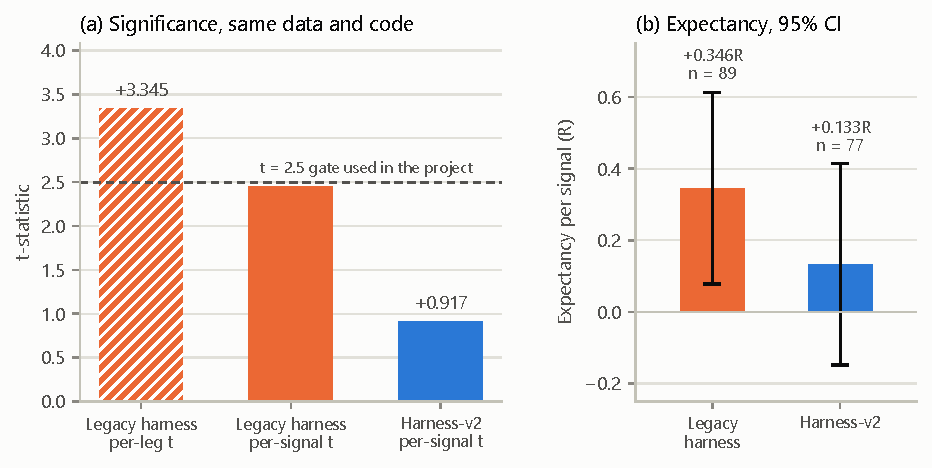
\includegraphics[width=\linewidth]{figures/F1_g0_calibration.pdf}
\caption{\csuse{capth-F1}}
\label{fig:F1}
\end{figure}

การนำการรั่วของข้อมูลอนาคตออกเพียงอย่างเดียว (จาก V1 เป็น V2) ทำให้ค่าสถิติ $t$ ต่อสัญญาณลดลงจาก $+2.453$
เหลือ $+0.917$ \tw{ค่าคาดหมาย}ต่อสัญญาณลดลง 62\% และกำไรสุทธิหายไป 69\% % [C07, C08, C12, C13]
ในการรันแบบเดิม การนับขาแทนการนับสัญญาณทำให้ค่า $t$ สูงเกินจริงขึ้นไปอีก 1.36 เท่า
(3.345 เทียบกับ 2.453) % [C11]
การลดลงสูงสุดไม่ได้ลดลงตาม\tw{ค่าคาดหมาย} (\tw{ภาพที่}~\ref{fig:F2}) ภายใต้ระบบที่แก้ไขแล้ว
\tw{หลักฐาน}ของความได้เปรียบคือสัญญาณ $n=77$ สัญญาณที่ $t=+0.92$ ซึ่ง\tw{ต่ำกว่า}ทุกเกณฑ์ที่ใช้ในโครงการ
และช่วงความเชื่อมั่น 95\% ของ\tw{ค่าคาดหมาย}ครอบคลุมศูนย์ นี่คือ\tw{หลักฐาน}หลักเกี่ยวกับกลยุทธ์\tw{ออร์เดอร์บล็อก}

\begin{figure}[htbp]
\centering
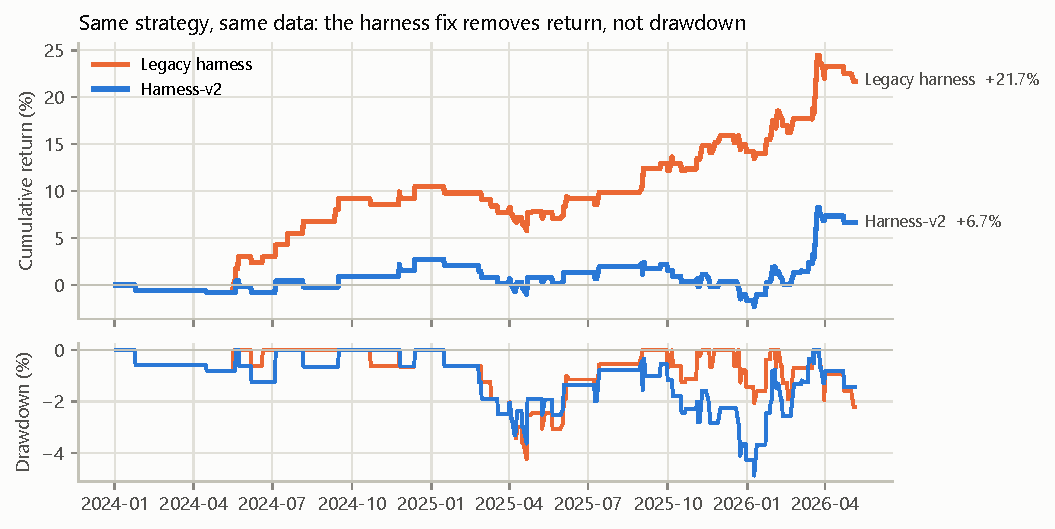
\includegraphics[width=\linewidth]{figures/F2_g0_equity.pdf}
\caption{\csuse{capth-F2}}
\label{fig:F2}
\end{figure}

\subsection{กลยุทธ์\tw{ออร์เดอร์บล็อก}: การวัดซ้ำภายในช่วงข้อมูลในตัวอย่าง}
\label{sec:res-remeasure}

เอกสารก่อนหน้าของโครงการรายงานว่า การปรับปรุงกลยุทธ์ที่ดูดีที่สุด---คือสัญญาณที่มี ``timing'' flag
\tw{อย่างน้อย}สองตัว---``ล่มสลายนอกตัวอย่าง'' (collapsed out of sample) ในที่นี้รายงานการเปรียบเทียบนั้นใหม่
ด้วยหน่วยที่ถูกต้องและคำอธิบายที่ตรงตามจริง การเปรียบเทียบนี้\emph{ไม่ใช่}การทดสอบนอกตัวอย่าง
\begin{itemize}
\item ตัวเลขในตัวอย่างมาจากการรันตลอดช่วงข้อมูล (ธันวาคม 2024 ถึงพฤษภาคม 2026)
ตัวเลขที่ใช้เปรียบเทียบมาจากหน้าต่างสั้น ๆ ห้าหน้าต่างระหว่างกุมภาพันธ์ 2025 ถึงเมษายน 2026
ซึ่งรัน\tw{ภายหลัง}ด้วยโค้ดรุ่นใหม่กว่าโดยไม่คิดต้นทุนการ\tw{ซื้อขาย} ทั้งห้าหน้าต่างอยู่ภายในช่วงข้อมูลในตัวอย่าง % [C36, C37, C65]
\item การปรับปรุงนี้ถูกเลือกหลังจากเห็นผลในตัวอย่างแล้ว
\item การรันทั้งสอง\tw{เกิดขึ้น}ก่อนการแก้ไขระบบทดสอบ จึงมีการรั่วของข้อมูลอนาคตทั้งคู่ % [C38]
\end{itemize}

เมื่อวัดต่อสัญญาณทั้งสองฝั่ง การปรับปรุงนี้เปลี่ยนจาก $t=+3.045$ ($n=228$) ในตัวอย่าง
เป็น $t=+0.06$ ($n=37$) ในหน้าต่างที่รันซ้ำ ส่วนกลุ่มสัญญาณทั้งหมดเปลี่ยนจาก $+2.18$ ($n=514$)
เป็น $+0.63$ ($n=43$) % [C30, C31, C34]
การวัดซ้ำนี้มีอำนาจการทดสอบต่ำ หากอัตราส่วน\tw{ชาร์ป}ต่อสัญญาณในตัวอย่าง
($3.045/\sqrt{228}\approx0.20$) เป็นค่าจริง ค่า $t$ ที่คาดไว้ที่ $n=37$ จะอยู่ที่ประมาณ
$0.20\sqrt{37}\approx1.2$ และค่าที่สังเกตได้ $+0.06$ อยู่\tw{ต่ำกว่า}ค่านั้นประมาณหนึ่งค่าความ\tw{คลาดเคลื่อน}มาตรฐาน
ซึ่งยังอยู่ในแถบของผลลัพธ์ที่สอดคล้องกับผลที่มีอยู่จริง (\tw{ภาพที่}~\ref{fig:F7})
การเปรียบเทียบนี้เพียงลำพังจึงเป็น\tw{หลักฐาน}ที่อ่อนในการคัดค้านการปรับปรุงดังกล่าว

เพื่อความครบถ้วน การทดสอบแบบเดินหน้าแบบยึดจุดเริ่มต้น (anchored walk-forward) บนระบบทดสอบแบบเดิม
(คะแนนขั้นต่ำ 75 และสถิติต่อขา) ให้ผลเป็นบวกในหน้าต่างทดสอบหกเดือนทั้งสามหน้าต่าง โดยมีค่า $t$ เท่ากับ
$+1.62$, $+1.02$ และ $+2.91$ และไม่มีหน้าต่างใดถึง 3.0 % [C39, C41]
การทดสอบแบบเดินหน้าที่คิดต้นทุนซึ่งรัน\tw{ภายหลัง} ไม่ถึง $t=2.5$ ในหน้าต่างใดเลยจากสามหน้าต่าง % [C40]
การรันทั้งสองมีการรั่วของข้อมูลอนาคต

\begin{figure}[htbp]
\centering
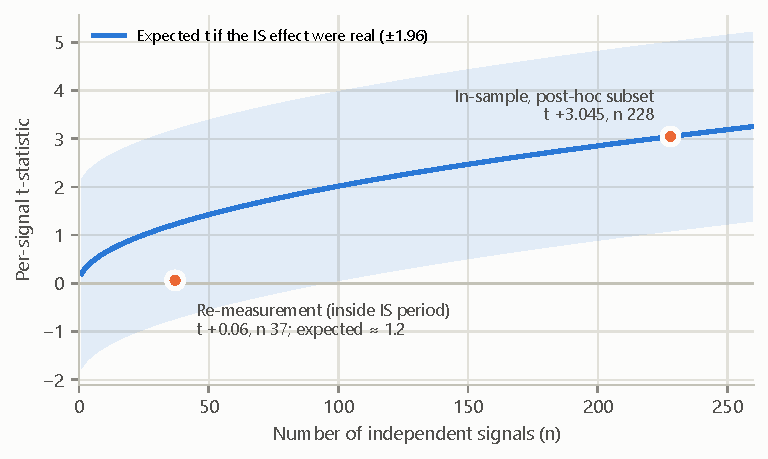
\includegraphics[width=0.78\linewidth]{figures/F7_power_band.pdf}
\caption{\csuse{capth-F7}}
\label{fig:F7}
\end{figure}

\subsection{กลยุทธ์โซนอุปสงค์--อุปทาน: ขั้นการพัฒนา}
\label{sec:res-zone}

ข้อกำหนดที่ตรึงไว้ (การทดลองที่~1) และรูปแบบที่ปรับเปลี่ยนอีกสามแบบถูกรันบนชุดข้อมูล DEV
(\tw{ตารางที่}~\ref{tab:zone} และ\tw{ภาพที่}~\ref{fig:F4}) การทดลองที่~2--4 ถูกเลือกหลังการทดลองที่~1
ภายใต้ข้อกำหนดที่อนุญาตให้ปรับแต่งบนชุด DEV ได้ และทั้งสี่การทดลองยังคงให้ผลติดลบ
การทดลองเหล่านี้เปลี่ยนพารามิเตอร์สองตัวที่ควบคุมคุณภาพของโซนโดยตรงที่สุด
คือเกณฑ์แรงเคลื่อนตัว (impulse) และอายุสูงสุดของโซน

\begin{table}[htbp]
\centering\small
\caption{กลยุทธ์โซนบนชุดข้อมูล DEV (2024) วัดต่อสัญญาณ คิดต้นทุน ความเสี่ยง 0.5\%
ตรงกับแถวที่ 1--4 ของสมุดบันทึกการทดลอง}
\label{tab:zone}
\begin{tabular}{@{}llrrrrrr@{}}
\toprule
การทดลอง & รูปแบบ & $n$ & PF & $E[\R]$ & $t$ (กำไร) & $t$ ($\R$) & DD สูงสุด (\%) \\
\midrule
1 & ตรึงไว้ v1.0 & 406 & 0.745 & $-0.143$ & $-2.79$ & $-2.92$ & 29.8 \\ % [C21]
2 & impulse $2.0\times$ATR & 240 & 0.772 & $-0.126$ & $-1.90$ & $-1.94$ & 17.4 \\ % [C22]
3 & อายุสูงสุด 24 แท่ง & 334 & 0.775 & $-0.124$ & $-2.21$ & $-2.28$ & 22.6 \\ % [C23]
4 & ทั้งสองอย่าง & 187 & 0.744 & $-0.141$ & $-1.92$ & $-1.92$ & 13.4 \\ % [C24]
\bottomrule
\end{tabular}
\end{table}

\begin{figure}[htbp]
\centering
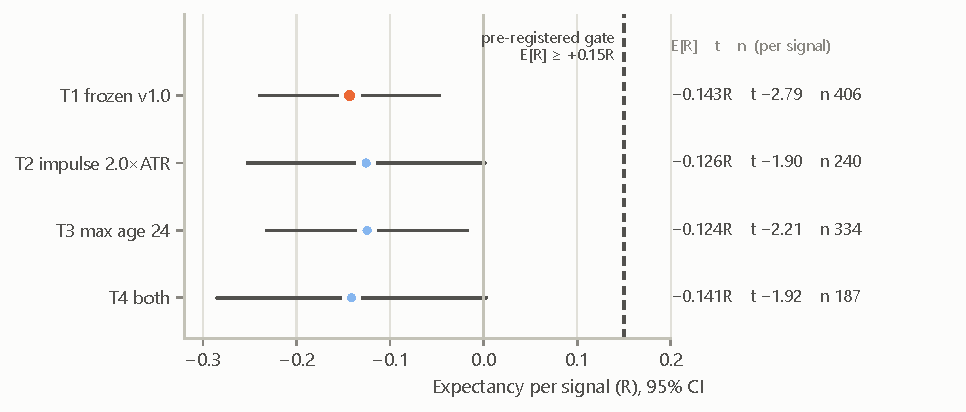
\includegraphics[width=0.92\linewidth]{figures/F4_zone_dev.pdf}
\caption{\csuse{capth-F4}}
\label{fig:F4}
\end{figure}

ข้อกำหนดที่ตรึงไว้อยู่ห่างจากเกณฑ์มาก ได้แก่ $t=-2.79$ เทียบกับ $+2.5$ \tw{ค่าคาดหมาย}
$-0.143\R$ เทียบกับ $+0.15\R$ และการลดลงสูงสุด 29.8\% เทียบกับ 6\% % [C19, C21]
ช่วงความเชื่อมั่น 95\% ของ\tw{ค่าคาดหมาย}ของข้อกำหนดนี้ไม่ครอบคลุมศูนย์
ส่วนช่วงของการทดลองที่~2 และ~4 มีขอบบนแตะศูนย์พอดี % [C75]
การวินิจฉัยสามประการอธิบายผลขาดทุน ดังนี้
\begin{itemize}
\item \textbf{ทิศทาง} ทั้งสองฝั่งขาดทุน สัญญาณขาย 208 สัญญาณและสัญญาณซื้อ 198 สัญญาณต่างมีกำไรเฉลี่ยติดลบ
ในปีที่ราคาทองคำปรับตัวขึ้นอย่างแรง ผลขาดทุนจึงไม่ได้เกิดจากการรับความเสี่ยงตามทิศทางของแนวโน้ม % [C25]
\item \textbf{ต้นทุน} ค่าคอมมิชชันและค่าธรรมเนียมข้ามคืน (swap) คิดเป็นประมาณ $-0.018\R$ จาก $-0.143\R$
หากไม่มีต้นทุนเหล่านี้ \tw{ค่าคาดหมาย}จะยังคงอยู่ที่ประมาณ $-0.125\R$ % [C27]
\item \textbf{คุณภาพ} การเข้มงวดพารามิเตอร์คุณภาพทั้งสองตัวลดจำนวนสัญญาณจาก 406 เหลือ 187
แต่\tw{ค่าคาดหมาย}ยังอยู่ระหว่าง $-0.14\R$ ถึง $-0.12\R$ หากการแตะโซนที่แข็งแรงกว่ามีความได้เปรียบ
\tw{ตัวกรอง}ที่เข้มงวดขึ้นควรทำให้ความได้เปรียบนั้นเด่นชัดขึ้น แต่ผลไม่เป็นเช่นนั้น % [C21–C24]
\end{itemize}
จากแท่ง H1 จำนวน 5,912 แท่ง มี 1,595 แท่งที่เกิดจุดกลับตัว (swing) เกิดโซนที่ใช้งานได้ 656 โซน
มีโซนถูกแตะ 508 โซน และมีการเข้า\tw{ซื้อขาย} 406 สัญญาณ (\tw{ภาพที่}~\ref{fig:F5}) % [C28]

ตามกฎการไม่ผ่านเกณฑ์ของข้อกำหนด การศึกษาหยุดที่ขั้นนี้ ชุดข้อมูล EVAL และ FRESH ไม่ได้ถูกใช้
และสมุดบันทึกมีสี่แถว % [C20, C29]

\begin{figure}[htbp]
\centering
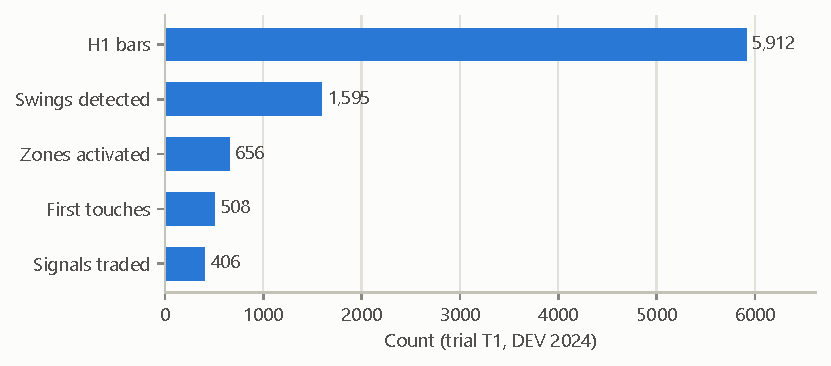
\includegraphics[width=0.7\linewidth]{figures/F5_zone_funnel.pdf}
\caption{\csuse{capth-F5}}
\label{fig:F5}
\end{figure}

\subsection{ทะเบียน\tw{แนวคิดที่}มีเอกสารยืนยัน}
\label{sec:res-register}

\tw{ตารางที่}~\ref{tab:ideas} แสดงทุก\tw{แนวคิดที่}มีไฟล์ผลต้นฉบับ หรือมีบันทึกที่ลงวันที่ไว้ในขณะนั้น
(\tw{ภาพที่}~\ref{fig:F6}) บันทึกของโครงการกล่าวถึงจำนวน\tw{แนวคิดที่}มากกว่านี้ คือประมาณสิบเก้าแนวคิด
แต่ไม่สามารถสร้างจำนวนนั้นขึ้นใหม่จากไฟล์ต้นฉบับได้ จึงแสดงเฉพาะ 15 \tw{แนวคิดที่}มีเอกสารยืนยัน
ป้ายระบุระดับ\tw{หลักฐาน} (\tw{คงไว้}เป็น\tw{ภาษาอังกฤษ}ให้ตรงกับภาพ) มีความหมายดังนี้
\textsc{Falsified} (ถูกหักล้าง): เกณฑ์ที่ลงทะเบียนไว้\tw{ล่วงหน้า}ไม่ผ่าน และค่าประมาณอยู่ผิดฝั่งอย่างมีนัยสำคัญ
หรือการไม่ผ่านเกณฑ์นั้นชัดเจนโดยไม่มี\tw{ข้อกำกวม}
\textsc{Not supported} (ไม่\tw{ได้รับ}การสนับสนุน): ทดสอบแล้ว แต่\tw{หลักฐาน}ของความได้เปรียบไม่ถึงเกณฑ์
\textsc{Inconclusive} (\tw{สรุปไม่ได้}): วัดแล้ว แต่ผลไม่สามารถแยกแยะได้
\textsc{Not tested} (ยังไม่ได้ทดสอบ): มี\tw{เครื่องมือ}แล้ว แต่ยังไม่มีผล
\tw{แนวคิดที่}ระบุว่า ``บันทึกไว้ ไม่ได้รันซ้ำ'' (recorded, not re-run) อิงบันทึกที่ลงวันที่ไว้
ซึ่งมี\tw{สคริปต์}ที่สร้างผลอยู่ แต่ไม่ได้บันทึกผลลัพธ์ไว้ และไม่ได้รันซ้ำสำหรับรายงานนี้

{\small
\begin{longtable}{@{}p{0.45cm}>{\raggedright\arraybackslash}p{3.6cm}>{\raggedright\arraybackslash}p{6.15cm}>{\raggedright\arraybackslash}p{3.0cm}@{}}
\caption{ทะเบียน\tw{แนวคิดที่}มีเอกสารยืนยัน 15 แนวคิด $\dagger$ = บันทึกไว้ ไม่ได้รันซ้ำ}\label{tab:ideas}\\
\toprule
\# & แนวคิด & ผลสำคัญ & ป้าย \\
\midrule
\endfirsthead
\toprule
\# & แนวคิด & ผลสำคัญ & ป้าย \\
\midrule
\endhead
1 & การประกอบกันของ\tw{ออร์เดอร์บล็อก} (ตรึงไว้) & ระบบที่แก้ไขแล้ว: $t=+0.92$ ต่อสัญญาณ, $n=77$ & \textsc{Not supported} \\ % [C07, C08]
2 & การปรับปรุง\tw{ออร์เดอร์บล็อก}แบบ $\geq$2 flag & $t=+3.045$ ($n=228$, เลือก\tw{ภายหลัง}) $\rightarrow$ $+0.06$ ($n=37$) เป็นการวัดซ้ำภายในช่วงในตัวอย่าง & \textsc{Not supported} \\ % [C31, C34]
3 & โซนอุปสงค์--อุปทาน v1.0 & DEV: $t=-2.79$, $E[\R]=-0.143$, $n=406$ & \textsc{Falsified} \\ % [C21]
4 & การส่ง\tw{คำสั่ง}แบบ pending limit & เกณฑ์ไม่ผ่าน: PF ของ limit 1.599 \tw{ต่ำกว่า} PF ของ\tw{คำสั่ง}ตลาด 1.718 & \textsc{Not supported} \\ % [C44]
5 & การเข้า\tw{ซื้อขาย}รายชั่วโมงด้วย limit order$\dagger$ & $t=1.98$ จากการจับคู่ 12 ครั้ง \tw{ต่ำกว่า} 2.5 & \textsc{Not supported} \\ % [C45]
6 & \tw{ตัวกรอง}สภาวะตลาดแบบ Hidden Markov & ผ่านเกณฑ์ Sharpe ที่ลงทะเบียนไว้\tw{ล่วงหน้า}ของตนเอง; 0 จาก 3 หน้าต่างถึง $t=2.5$; ระบบทดสอบแบบเดิม & \textsc{Inconclusive} \\ % [C43]
7 & \tw{ตัวกรอง}การ\tw{ซื้อขาย}ด้วยโมเดลภาษา$\dagger$ & อนุมัติการ\tw{ซื้อขาย} 11 ครั้ง, $p=1.00$ & \textsc{Inconclusive} \\ % [C49]
8 & การเรียนรู้ของเครื่องบนคุณลักษณะราคา M15$\dagger$ & AUC 0.491--0.503; ตัวควบคุมเชิงบวก 0.693 & \textsc{Not supported} \\ % [C46]
9 & \tw{ส่วนชดเชย}ความเสี่ยงด้านความผันผวน (volatility risk premium)$\dagger$ & ความผันผวนแฝงสูงกว่าความผันผวนที่\tw{เกิดขึ้น}จริง 4.05 จุดใน 85.3\% ของวัน; เดือนที่แย่ที่สุด $-309\%$ & \textsc{Not supported}\textsuperscript{a} \\ % [C47]
10 & ความไม่สมดุลของ\tw{คำสั่ง}\tw{ซื้อขาย}คริปโต$\dagger$ & สุทธิ $-2.80$ ถึง $-4.05$ basis point ต่อการ\tw{ซื้อขาย} & \textsc{Not supported} \\ % [C48]
11 & คู่สินทรัพย์ที่มีความสัมพันธ์ระยะยาว (cointegration) (16 คู่) & 0 จาก 16 คู่ผ่านการทดสอบ FDR, frozen-$\beta$ และ half-life & \textsc{Falsified} \\ % [C50]
12 & \tw{โมเมนตัม}ภาคตัดขวางของคริปโต$\dagger$ & Deflated Sharpe 0.21 ที่จำนวนการทดลองตามจริง & \textsc{Falsified} \\ % [C51]
13 & \tw{โมเมนตัม}อนุกรมเวลาแบบ\tw{พอร์ต} (41 สินทรัพย์) & ผ่านระยะที่ 1 (Deflated Sharpe 0.982, $N=86$); ไม่มี alpha ที่มีนัยสำคัญเหนือ ETF ประเภท managed futures ($p=0.068$) & \textsc{Not supported}\textsuperscript{b} \\ % [C52, C53]
14 & การเก็งกำไรแบบตะกร้าในตลาดพยากรณ์ (prediction market) & มีเพียงข้อมูล ณ จุดเวลาหนึ่ง (snapshot) ยังไม่มีข้อสรุป & \textsc{Not tested} \\ % [C54]
15 & การให้คะแนนโซนที่บุคคลภายนอกโพสต์ & สร้างและทดสอบตัวให้คะแนนแล้ว แต่ไม่เคย\tw{ได้รับ}ข้อมูล & \textsc{Not tested} \\ % [C55]
\bottomrule
\multicolumn{4}{@{}p{14cm}@{}}{\footnotesize\RaggedRight \textsuperscript{a}พบ\tw{ส่วนชดเชย}ความเสี่ยง
แต่ความเสี่ยงส่วนหางไม่สอดคล้องกับเพดานการลดลงของมูลค่า 10\% \textsuperscript{b}พบ\tw{ส่วนชดเชย}ความเสี่ยง
แต่ไม่มีนัยสำคัญเหนือกองทุน managed futures ที่\tw{ซื้อขาย}ในตลาด (ไม่รวมคริปโต $p=0.156$)}\\
\end{longtable}
}

\begin{figure}[htbp]
\centering
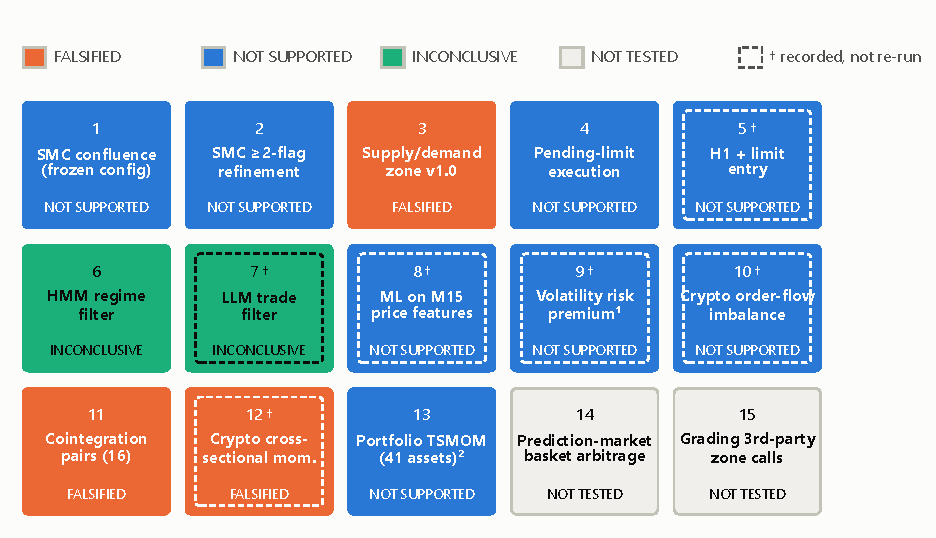
\includegraphics[width=0.9\linewidth]{figures/F6_idea_register.pdf}
\caption{\csuse{capth-F6}}
\label{fig:F6}
\end{figure}

% ════════════════════════════════════════════════════════════════════════════
\FloatBarrier
\section{อภิปรายผล}
\label{sec:discussion}

\subsection{สิ่งที่\tw{หลักฐาน}แสดง}
ภายใต้ระบบทดสอบที่ใช้เฉพาะข้อมูล ณ เวลา\tw{ตัดสินใจ}และการอนุมานต่อสัญญาณ กฎโครงสร้างราคาทั้งสองกลุ่ม
ไม่แสดงความได้เปรียบต่อสัญญาณที่วัดได้บนสินทรัพย์และช่วงเวลานี้ ผลทั้งสองต่างกันโดยลักษณะ
ผลของ\tw{ออร์เดอร์บล็อก}เป็นผลว่าง (null) คือค่าประมาณแบบจุดเป็นบวก แต่ช่วงความเชื่อมั่นครอบคลุมศูนย์
ส่วนผลของโซนติดลบอย่างมีนัยสำคัญภายใต้ข้อกำหนดที่ตรึงไว้ สมมาตรระหว่างฝั่งซื้อและฝั่งขาย
ไม่ได้อธิบายได้ด้วยต้นทุน และไม่ตอบสนองต่อ\tw{ตัวกรอง}คุณภาพซึ่งหลักคิดของกลยุทธ์บอกว่าควรมีผล

\subsection{สิ่งที่\tw{หลักฐาน}ไม่ได้แสดง}
\tw{หลักฐาน}ไม่ได้แสดงว่ากฎเหล่านี้ใช้ไม่ได้ในที่อื่น เพราะศึกษาเพียงสินทรัพย์เดียว ผู้ให้ข้อมูลรายเดียว
และช่วงเวลาเดียว อีกทั้งกลยุทธ์โซนถูกประเมินบนชุดข้อมูลสำหรับการพัฒนาเท่านั้น
\tw{หลักฐาน}ไม่ได้แสดงว่ากลยุทธ์\tw{ออร์เดอร์บล็อก}มีความได้เปรียบเป็นศูนย์
แสดงเพียงว่า\tw{หลักฐาน}ของความได้เปรียบ\tw{ต่ำกว่า}เกณฑ์ที่สมเหตุสมผลใด ๆ อยู่มาก
และการวัดซ้ำภายในช่วงในตัวอย่างใน\tw{ส่วนที่}~\ref{sec:res-remeasure} เป็น\tw{หลักฐาน}ที่อ่อนทั้งสองทาง

\subsection{ข้อบกพร่องของระบบทดสอบทำให้ค่าเฉลี่ยสูงเกินจริง ไม่ใช่ความแปรปรวน}
ในการปรับเทียบ \tw{ค่าคาดหมาย}ลดลง 62\% ขณะที่การลดลงสูงสุดยังอยู่ใกล้ 5\% (\tw{ตารางที่}~\ref{tab:g0})
การรั่วของข้อมูลอนาคตทำให้\emph{การเลือกและผลลัพธ์}ของการ\tw{ซื้อขาย}ดีขึ้น---ซึ่งเป็นตัวเศษของค่าสถิติ $t$---
ขณะที่การ\tw{กระจาย}ของผลลัพธ์แทบไม่เปลี่ยนแปลง นัยสำคัญที่สูงมากในตัวอย่าง
ควบคู่กับการลดลงของมูลค่าในระดับปกติ เป็นรูปแบบที่ควร\tw{ตรวจสอบ}

\subsection{การรั่วของข้อมูลอนาคตไม่สามารถอธิบายช่องว่างระหว่างผลในตัวอย่างกับผลการวัดซ้ำได้}
ทั้งสองฝั่งของการเปรียบเทียบใน\tw{ส่วนที่}~\ref{sec:res-remeasure} รันบนระบบทดสอบแบบเดิม
การรั่วของข้อมูลอนาคตจึงส่งผลต่อทั้งสองฝั่ง และไม่สามารถอธิบายความแตกต่างระหว่างกันได้ % [C38]
คำอธิบายที่ประหยัดกว่าคืออคติจากการคัดเลือก การปรับปรุงนี้ถูกเลือกหลังเห็นผลในตัวอย่าง
จากคะแนนที่ในทางปฏิบัติแปรผันเพียงมิติเดียว เนื่องจาก flag ห้าในหกตัวของคะแนนนี้
แทบจะเปิดอยู่เสมอหรือปิดอยู่เสมอในกลุ่มสัญญาณที่ถูก\tw{ซื้อขาย} (บันทึกไว้ ไม่ได้รันซ้ำ) % [C42]
การวัดซ้ำมีขนาดเล็กเกินกว่าจะแยกอคติจากการคัดเลือกออกจากผลที่มีอยู่จริงแต่มีสัญญาณรบกวนสูงได้
ข้อสรุปจึงอาศัยการปรับเทียบด้วยระบบที่แก้ไขแล้ว

\subsection{ความสัมพันธ์กับวรรณกรรมเรื่องการกระจุกตัวของ\tw{คำสั่ง}\tw{ซื้อขาย}}
\tw{หลักฐาน}จากข้อมูล\tw{คำสั่ง}\tw{ซื้อขาย}ของ \citet{osler2003currency,osler2005stoploss}
เกี่ยวกับระดับราคาที่มีเอกสารยืนยันว่ามี\tw{คำสั่ง}รออยู่ รายงานนี้ไม่ได้แสดงว่า\tw{ออร์เดอร์บล็อก}
และโซนที่นักลงทุน\tw{รายย่อย}ลากขึ้นตรงกับระดับดังกล่าว การทดสอบโซนวัดผลตอบแทนของการเข้า\tw{ซื้อขาย}
เมื่อราคาแตะโซนโดยตรง และพบว่าติดลบ ซึ่งเป็นผลที่คาดได้หากระดับที่ลากขึ้น
ไม่ใช่ที่ที่\tw{คำสั่ง}ฝั่งตรงข้ามรออยู่จริง

\subsection{การแก้ไขเอกสารก่อนหน้าของโครงการ}
\label{sec:corrections}
รายงานนี้แก้ไขข้อความสามข้อในเอกสารก่อนหน้าของโครงการ เอกสารต้นฉบับยังคงเดิมทุกประการ
และการแก้ไขถูกบันทึกเป็นบันทึกใหม่ที่ลงวันที่
\begin{enumerate}
\item \textbf{หน่วยไม่ตรงกัน} ข้อความ ``in-sample $t=+3.05$, out-of-sample $t=+0.09$''
เปรียบเทียบสถิติต่อสัญญาณในตัวอย่างกับสถิติต่อขาจากหน้าต่างที่ใช้เปรียบเทียบ
เมื่อวัดต่อสัญญาณทั้งสองฝั่ง ตัวเลขคือ $+3.045$ และ $+0.06$ % [C35]
\item \textbf{ระบุผิดว่าเป็นการทดสอบนอกตัวอย่าง} หน้าต่างที่ใช้เปรียบเทียบอยู่ภายในช่วงข้อมูลในตัวอย่าง
รันด้วยโค้ดรุ่นใหม่กว่าโดยไม่คิดต้นทุน และเป็นหน้าต่างสั้น ๆ ที่เลือกเฉพาะกิจ
ไม่ใช่รอบของการทดสอบแบบเดินหน้า การเปรียบเทียบนี้จึงเป็นการวัดซ้ำภายในช่วงในตัวอย่าง % [C36, C37]
\item \textbf{ป้ายการตั้งค่า} บันทึกการทดสอบแบบเดินหน้าฉบับหนึ่งระบุคะแนนขั้นต่ำเป็น 65
แต่ไฟล์ผลแสดงว่าไม่มีการ\tw{ซื้อขาย}ที่คะแนน\tw{ต่ำกว่า} 75 เลย
ซึ่งสอดคล้องกับการเปลี่ยนการตั้งค่าที่ลงวันที่ไว้สามวันก่อนการรัน % [C41]
\end{enumerate}

% ════════════════════════════════════════════════════════════════════════════
\section{ข้อจำกัด}
\label{sec:limits}

\begin{itemize}
\item \textbf{สินทรัพย์เดียว แหล่งข้อมูลเดียว} ศึกษาเฉพาะ XAUUSD โดยใช้ราคาเสนอซื้อ (BID) จาก Dukascopy
ข้อมูลราคาของ\tw{โบรกเกอร์}แต่ละรายต่างกันทั้งในด้านส่วนต่างราคา (spread) และป้ายเวลา % [C63]
\item \textbf{การจำลองการจับคู่\tw{คำสั่ง}จากแท่งราคา} การออกจากสถานะถูกตัดสินจากราคาสูงสุดและต่ำสุดของแท่ง
เมื่อทั้งจุดตัดขาดทุนและจุดทำกำไรถูกแตะภายในแท่งเดียวกัน จะสมมติว่าจุดตัดขาดทุนถูกแตะก่อน
แท่งที่เปิดเลยระดับใดระดับหนึ่งไปแล้วจะจับคู่ที่ราคาเปิด ลำดับที่แท้จริงภายในแท่งไม่เป็นที่รู้ % [C66]
\item \textbf{ข้อมูลที่ใช้ในระบบจริงและในการทดสอบย้อนหลังต่างกัน} ข้อมูลที่ระบบจริง\tw{ได้รับ}รวมแท่งปัจจุบันที่ยังไม่ปิด
และกลยุทธ์อ่านค่าล่าสุดของแท่งนั้น ขณะที่การทดสอบย้อนหลังที่แก้ไขแล้วใช้เฉพาะแท่งที่ปิดแล้ว
การทดสอบย้อนหลังจึงไม่ได้จำลองกฎการ\tw{ตัดสินใจ}ของระบบจริงอย่างตรงทุกประการ
และยังไม่ได้วัดทิศทางและขนาดของผลกระทบต่อผลลัพธ์ % [C67]
\item \textbf{สมุดบันทึกการทดลองเริ่มช้า} สมุดบันทึกเริ่มพร้อมกับการศึกษากลยุทธ์โซน
งานด้าน\tw{ออร์เดอร์บล็อก}ก่อนหน้านั้นได้ลองการตั้งค่าจำนวนมากที่ไม่ได้บันทึกไว้
ดังนั้นอัตราส่วน\tw{ชาร์ป}แบบปรับลดใด ๆ ที่คำนวณสำหรับงานนั้นด้วย $N$ ขนาดเล็กจึงให้\tw{ภาพที่}ดีเกินจริง
\item \textbf{ยังไม่ได้วัดตัวควบคุมและต้นทุนในการ\tw{ซื้อขาย}จริง} ยังไม่ได้รันตัวควบคุมเชิงศูนย์บนระบบที่แก้ไขแล้ว
ยังไม่ได้วัดต้นทุนและค่า\tw{คลาดเคลื่อน}ของราคาในการ\tw{ซื้อขาย}จริงเทียบกับสมมติฐานของการทดสอบย้อนหลัง
และการทดสอบ\tw{ล่วงหน้า}บนบัญชีทดลองมีการ\tw{ซื้อขาย}ประมาณ 0 จาก 30 ครั้งที่กำหนด % [C56]
\item \textbf{บันทึกที่ไม่ได้รันซ้ำ} แนวคิดหกแนวคิดใน\tw{ตารางที่}~\ref{tab:ideas}
อิงบันทึกที่ลงวันที่ไว้ซึ่งไม่ได้บันทึกผลลัพธ์ไว้
\item \textbf{ป้ายเวลาที่บันทึกเอง} ลำดับเวลาของการลงทะเบียน\tw{ล่วงหน้า}อาศัยเวลา commit ของระบบควบคุม\tw{เวอร์ชัน}
ที่บันทึกโดยเครื่องของผู้เขียนเอง ซึ่งไม่\tw{ได้รับ}การรับรองจากบุคคลภายนอก % [C68]
\item \textbf{การพัฒนาโดยมีผู้ช่วย AI} ซอฟต์แวร์และการวิเคราะห์ถูกพัฒนาด้วยผู้ช่วยเขียนโค้ด AI
ดูการเปิดเผยข้อมูลใน\tw{ภาคผนวก}~\ref{app:disclosure}
\end{itemize}

% ════════════════════════════════════════════════════════════════════════════
\section{สรุป}

บนข้อมูล XAUUSD ราย 5 นาที รายงานนี้\tw{ตรวจสอบ}กฎโครงสร้างราคาของนักลงทุน\tw{รายย่อย}สองกลุ่ม
ภายใต้การทดสอบย้อนหลังที่ใช้เฉพาะข้อมูล ณ เวลา\tw{ตัดสินใจ}และการอนุมานต่อสัญญาณ
ความได้เปรียบที่ปรากฏของกลยุทธ์\tw{ออร์เดอร์บล็อก}ส่วนใหญ่เป็นผลจากข้อบกพร่องสองประการของระบบทดสอบ
เมื่อแก้ไขบนข้อมูลและโค้ดชุดเดียวกัน ค่าสถิติ $t$ ต่อสัญญาณลดลงจาก $+2.45$ เหลือ $+0.92$
กลยุทธ์โซนอุปสงค์--อุปทาน ซึ่งกำหนดและ commit ข้อกำหนดไว้ก่อนผลการทดสอบย้อนหลัง\tw{ครั้งแรก}
ไม่ผ่านเกณฑ์ที่ลงทะเบียนไว้\tw{ล่วงหน้า}ตั้งแต่ขั้นการพัฒนา โดยมี\tw{ค่าคาดหมาย}ติดลบอย่างมีนัยสำคัญ
และข้อมูลสำหรับการประเมินผลไม่ได้ถูกใช้ ผลทั้งสองไม่สนับสนุนการ\tw{ซื้อขาย}ตามกฎเหล่านี้
ผลลัพธ์ที่คงทนของโครงการคือ\tw{เครื่องมือ}\tw{ตรวจสอบ}ความถูกต้อง---การตัดหน้าต่างข้อมูลตามเวลาปิดของแท่ง
พร้อมการทดสอบบังคับ สถิติต่อสัญญาณ และสมุดบันทึกการทดลองแบบเพิ่มได้อย่างเดียว---
และแนวปฏิบัติในการวัดแนวคิดก่อนที่จะเชื่อ

% ════════════════════════════════════════════════════════════════════════════
\FloatBarrier
\bibliographystyle{plainnat}
\bibliography{references_verified}

\appendix
\section{การทำซ้ำผลการศึกษา}
\label{app:repro}

\subsection{แผนผังไฟล์}
ชุด\tw{หลักฐาน}สาธารณะมีโครงสร้างเดียวกับโครงการ กลุ่มหลักมีดังนี้
\begin{itemize}[before=\RaggedRight]
\item \texttt{report\_calib\_v1\_full.json}, \texttt{report\_calib\_v2\_full.json}: การรันปรับเทียบ
(\tw{ตารางที่}~\ref{tab:g0}); \texttt{report\_costs\_065.json}: ไฟล์ผลแบบเดิมที่บันทึกไว้
\item \texttt{report\_zone\_dev\_t1.json}--\texttt{t4.json}, \texttt{trials.csv},
\texttt{specs/phase1\_zone\_spec\_v1.md}, \texttt{reports/phase2/DEV\_report.md}: การศึกษากลยุทธ์โซน
\item \texttt{report\_full.json}, \texttt{report\_w1.json}--\texttt{w5.json}: การวัดซ้ำภายในช่วงในตัวอย่าง;
\texttt{wfv\_*.json}: การทดสอบแบบเดินหน้า
\item \texttt{backtest/}, \texttt{quant/}, \texttt{core/}, \texttt{tools/}, \texttt{tests/}:
โค้ดที่สร้างผลลัพธ์ และโค้ดที่อ้างถึงในข้อจำกัด; \texttt{research/}: บันทึกของ\tw{แนวคิดที่} 11--14
(ผลของ cointegration ถูกเก็บสำเนาไว้ในคลังเก็บ จึงไม่มีการอ่านไฟล์นอกคลังเก็บระหว่างการสร้างรายงาน)
\item \texttt{paper/claims.csv}: ตัวเลขทุกตัวในรายงานนี้ พร้อมไฟล์ต้นทางและตำแหน่งในไฟล์
\end{itemize}

\subsection{การรันการ\tw{ตรวจสอบ}ซ้ำ}
ด้วยสภาพแวดล้อม Python ของโครงการ
\begin{itemize}[before=\RaggedRight]
\item \texttt{python -m tests.test\_no\_lookahead} (การทดสอบความเป็นเหตุเป็นผล 1,000 จุด);
\texttt{python -m tests.test\_per\_signal\_metrics}; \texttt{python -m tests.test\_zone\_engine};
\texttt{python -m tests.test\_zone\_runner}
\item \texttt{python backtest/\_flag\_analysis.py report\_w1.json \ldots{} report\_w5.json}
(\tw{ส่วนที่}~\ref{sec:res-remeasure} ทั้งต่อขาและต่อสัญญาณ)
\item \texttt{python -m backtest.zone\_cli} ด้วยพารามิเตอร์ใน \texttt{trials.csv}
(การทดลองกลยุทธ์โซน ทุกการรันจะเพิ่มแถวในสมุดบันทึก)
\item \texttt{python paper/figures/make\_figures.py --root .} (ภาพทั้งหมดและคำบรรยายภาพ
ไลบรารีที่ต้องใช้อยู่ใน \texttt{paper/requirements-figures.txt})
\item \texttt{data/\_fetch\_dukascopy\_2024.py} (ข้อมูลราคา ให้เทียบกับค่าแฮชด้านล่าง)
\end{itemize}
ในคลังเก็บสาธารณะ \texttt{tests.test\_no\_lookahead} และ \texttt{tests.test\_zone\_runner}
ต้องใช้ข้อมูลราคาหรือโมดูลการตั้งค่าของระบบจริง ซึ่งไม่ได้เผยแพร่ทั้งคู่ จึงถูกรายงานว่าข้าม (skipped)

\subsection{ค่าแฮชของไฟล์สาธารณะ}
ตารางแสดงค่าแฮช SHA-256 (16 หลักแรกของเลขฐานสิบหก ค่าเต็มอยู่ใน
\texttt{SHA256SUMS.txt}) ของทุกไฟล์ในชุด\tw{หลักฐาน}สาธารณะ มีไฟล์ที่ถูกปกปิดข้อมูลหกไฟล์
\textbf{การเปลี่ยนแปลงเพียงอย่างเดียวจากการปกปิดข้อมูลคือการแทนที่ชื่อ\tw{โฟลเดอร์}เดิมของโครงการด้วยคำว่า
\texttt{project}} ไฟล์สี่ไฟล์ไม่ได้เผยแพร่ และแสดงด้วยค่าแฮชของต้นฉบับ ได้แก่ ข้อมูลราคา
(ยังไม่ได้\tw{ตรวจสอบ}เงื่อนไขการเผยแพร่ซ้ำ) บันทึกการทดสอบด้วยการฉีดความผิดพลาดและบันทึกที่ลงวันที่หนึ่งฉบับ
ซึ่งมีรหัสระบุบัญชีทดลอง และไฟล์สถานะโครงการซึ่งระบุชื่อ\tw{โบรกเกอร์}และยอดเงินในบัญชี ค่าแฮชเต็มของไฟล์เหล่านี้อยู่ใน
\texttt{EXCLUDED.SHA256SUMS.txt} เพื่อให้ผู้อ่านที่สร้างข้อมูลราคาขึ้นใหม่\tw{ตรวจสอบ}ได้
\tw{สคริปต์}\tw{ตรวจสอบ}จะรายงานการ\tw{ตรวจสอบ}ที่ต้องใช้ไฟล์ที่ไม่ได้เผยแพร่ว่า\emph{ข้าม} (skipped)
และไม่นับว่าผ่านเมื่อไม่มีไฟล์นั้น

{\scriptsize
\begin{longtable}{@{}>{\raggedright\arraybackslash}p{8.6cm}p{2.7cm}>{\raggedright\arraybackslash}p{3.4cm}@{}}
\toprule
ไฟล์ & SHA-256 (ส่วนต้น) & สถานะ \\
\midrule
\endhead
\texttt{data/\allowbreak{}xauusd\_m5\_full.csv} & \texttt{86271f9b6fb4e3fd} & ไม่เผยแพร่ (ค่าแฮชของต้นฉบับ) \\
\texttt{data/\allowbreak{}\_fetch\_dukascopy\_2024.py} & \texttt{d4002cefd405685c} & ตรงตามต้นฉบับ \\
\texttt{trials.csv} & \texttt{8334fec3d4328530} & ตรงตามต้นฉบับ \\
\texttt{report\_costs\_065.json} & \texttt{0222ae8b91756bac} & ตรงตามต้นฉบับ \\
\texttt{bt\_costs\_065.log} & \texttt{db8526f5c1faaaaf} & ตรงตามต้นฉบับ \\
\texttt{report\_calib\_v1\_full.json} & \texttt{611cf0bbc7003970} & ตรงตามต้นฉบับ \\
\texttt{report\_calib\_v2\_full.json} & \texttt{c71ed4c181c1f610} & ตรงตามต้นฉบับ \\
\texttt{bt\_calib\_v1.err.log} & \texttt{fff56ea2769ced38} & ปกปิดข้อมูล (แทนที่ 2 จุด) \\
\texttt{bt\_calib\_v2.err.log} & \texttt{966a9abc0459bf5d} & ปกปิดข้อมูล (แทนที่ 30 จุด) \\
\texttt{reports/\allowbreak{}phase0/\allowbreak{}G0\_report.md} & \texttt{4af0b3a88a5079a3} & ปกปิดข้อมูล (แทนที่ 1 จุด) \\
\texttt{reports/\allowbreak{}phase0/\allowbreak{}diff\_0.1\_lookahead\_fix.patch} & \texttt{b4cf3193f6a59803} & ปกปิดข้อมูล (แทนที่ 6 จุด) \\
\texttt{reports/\allowbreak{}phase0/\allowbreak{}diff\_0.2\_per\_signal\_stats.md} & \texttt{0617b21a7b3d05d1} & ตรงตามต้นฉบับ \\
\texttt{reports/\allowbreak{}phase0/\allowbreak{}calib\_json\_sha256.txt} & \texttt{8978645fc696cf2f} & ตรงตามต้นฉบับ \\
\texttt{reports/\allowbreak{}phase0/\allowbreak{}report\_calib\_v1\_smoke.json} & \texttt{9416ed1809dbe99a} & ตรงตามต้นฉบับ \\
\texttt{reports/\allowbreak{}phase0/\allowbreak{}report\_calib\_v2\_smoke.json} & \texttt{9416ed1809dbe99a} & ตรงตามต้นฉบับ \\
\texttt{reports/\allowbreak{}phase0/\allowbreak{}bt\_calib\_v1\_attempt1\_crash.log} & \texttt{da988159c0276538} & ปกปิดข้อมูล (แทนที่ 11 จุด) \\
\texttt{specs/\allowbreak{}phase1\_zone\_spec\_v1.md} & \texttt{03ddb7b216a925c0} & ปกปิดข้อมูล (แทนที่ 1 จุด) \\
\texttt{reports/\allowbreak{}phase2/\allowbreak{}DEV\_report.md} & \texttt{f2a16fe6b48399b3} & ตรงตามต้นฉบับ \\
\texttt{report\_zone\_dev\_t1.json} & \texttt{8e78f735b0f4b135} & ตรงตามต้นฉบับ \\
\texttt{report\_zone\_dev\_t2.json} & \texttt{680cfa7bc39d4ac3} & ตรงตามต้นฉบับ \\
\texttt{report\_zone\_dev\_t3.json} & \texttt{cabb08e7febc8bc5} & ตรงตามต้นฉบับ \\
\texttt{report\_zone\_dev\_t4.json} & \texttt{3b6de201b05e0ac0} & ตรงตามต้นฉบับ \\
\texttt{report\_full.json} & \texttt{a7fedee66dc7badc} & ตรงตามต้นฉบับ \\
\texttt{report\_w1.json} & \texttt{8c76ed83a99772f3} & ตรงตามต้นฉบับ \\
\texttt{report\_w2.json} & \texttt{476833c1c1aa009c} & ตรงตามต้นฉบับ \\
\texttt{report\_w3.json} & \texttt{cd33449fc8eec236} & ตรงตามต้นฉบับ \\
\texttt{report\_w4.json} & \texttt{a849526720e1a6c8} & ตรงตามต้นฉบับ \\
\texttt{report\_w5.json} & \texttt{ecfc8198f9d91cf1} & ตรงตามต้นฉบับ \\
\texttt{report\_prefix.json} & \texttt{8898ed82d66324b9} & ตรงตามต้นฉบับ \\
\texttt{report\_postfix.json} & \texttt{8898ed82d66324b9} & ตรงตามต้นฉบับ \\
\texttt{wfv\_report.json} & \texttt{a3dc15dfa9f50c0b} & ตรงตามต้นฉบับ \\
\texttt{wfv\_baseline\_75.json} & \texttt{f07a8b665eda1e23} & ตรงตามต้นฉบับ \\
\texttt{wfv\_hmm\_report.json} & \texttt{d7879cef6fda776b} & ตรงตามต้นฉบับ \\
\texttt{report\_limit\_vs\_market.json} & \texttt{33d6801c11b06c4a} & ตรงตามต้นฉบับ \\
\texttt{tools/\allowbreak{}\_configB\_oos.json} & \texttt{36a77c746a8dd01d} & ตรงตามต้นฉบับ \\
\texttt{tools/\allowbreak{}\_configB\_exp4.json} & \texttt{ec0035833e3f6bd9} & ตรงตามต้นฉบับ \\
\texttt{research/\allowbreak{}tsmom\_portfolio/\allowbreak{}RESULTS.md} & \texttt{28b419edd88bf6f6} & ตรงตามต้นฉบับ \\
\texttt{research/\allowbreak{}tsmom\_portfolio/\allowbreak{}run\_log.txt} & \texttt{c9d2f84955210870} & ตรงตามต้นฉบับ \\
\texttt{research/\allowbreak{}tsmom\_portfolio/\allowbreak{}PHASE2\_SUMMARY.md} & \texttt{87320cdf3e460fa9} & ตรงตามต้นฉบับ \\
\texttt{research/\allowbreak{}tsmom\_portfolio/\allowbreak{}phase2\_run\_log.txt} & \texttt{37fa31cd3c22991d} & ตรงตามต้นฉบับ \\
\texttt{research/\allowbreak{}xs\_crypto\_momentum/\allowbreak{}RESULTS.md} & \texttt{48f4a492098dcd7a} & ตรงตามต้นฉบับ \\
\texttt{research/\allowbreak{}polymarket\_arb/\allowbreak{}snapshot\_existence.json} & \texttt{e1ce759409f3f4af} & ตรงตามต้นฉบับ \\
\texttt{.claude/\allowbreak{}skills/\allowbreak{}quant-\allowbreak{}trading/\allowbreak{}lessons/\allowbreak{}2026-\allowbreak{}05-\allowbreak{}29-\allowbreak{}walk-\allowbreak{}forward-\allowbreak{}results.md} & \texttt{155831b287b99313} & ตรงตามต้นฉบับ \\
\texttt{.claude/\allowbreak{}skills/\allowbreak{}quant-\allowbreak{}trading/\allowbreak{}lessons/\allowbreak{}2026-\allowbreak{}05-\allowbreak{}29-\allowbreak{}pending-\allowbreak{}limit-\allowbreak{}order-\allowbreak{}system.md} & \texttt{fc59a457d8ca53a4} & ตรงตามต้นฉบับ \\
\texttt{.claude/\allowbreak{}skills/\allowbreak{}quant-\allowbreak{}trading/\allowbreak{}lessons/\allowbreak{}2026-\allowbreak{}05-\allowbreak{}31-\allowbreak{}hmm-\allowbreak{}regime-\allowbreak{}detection.md} & \texttt{52ec0f7a8d5c3381} & ตรงตามต้นฉบับ \\
\texttt{.claude/\allowbreak{}skills/\allowbreak{}quant-\allowbreak{}trading/\allowbreak{}lessons/\allowbreak{}2026-\allowbreak{}06-\allowbreak{}03-\allowbreak{}phase0-\allowbreak{}execution-\allowbreak{}hardening.md} & \texttt{873ea28115830546} & ตรงตามต้นฉบับ \\
\texttt{.claude/\allowbreak{}skills/\allowbreak{}quant-\allowbreak{}trading/\allowbreak{}lessons/\allowbreak{}2026-\allowbreak{}06-\allowbreak{}05-\allowbreak{}llm-\allowbreak{}htf-\allowbreak{}demotion.md} & \texttt{6b8b50bf6cf8be20} & ไม่เผยแพร่ (ค่าแฮชของต้นฉบับ) \\
\texttt{.claude/\allowbreak{}skills/\allowbreak{}quant-\allowbreak{}trading/\allowbreak{}lessons/\allowbreak{}2026-\allowbreak{}06-\allowbreak{}10-\allowbreak{}backtest-\allowbreak{}on2-\allowbreak{}and-\allowbreak{}desync.md} & \texttt{1b7084b22b787ae6} & ตรงตามต้นฉบับ \\
\texttt{.claude/\allowbreak{}skills/\allowbreak{}quant-\allowbreak{}trading/\allowbreak{}lessons/\allowbreak{}2026-\allowbreak{}06-\allowbreak{}13-\allowbreak{}h1-\allowbreak{}limit-\allowbreak{}phase1.md} & \texttt{bc03bf3643d63957} & ตรงตามต้นฉบับ \\
\texttt{.claude/\allowbreak{}skills/\allowbreak{}quant-\allowbreak{}trading/\allowbreak{}lessons/\allowbreak{}2026-\allowbreak{}06-\allowbreak{}13-\allowbreak{}signal-\allowbreak{}rootcause-\allowbreak{}smc-\allowbreak{}degenerate.md} & \texttt{65e4c95cdd797ec3} & ตรงตามต้นฉบับ \\
\texttt{.claude/\allowbreak{}skills/\allowbreak{}quant-\allowbreak{}trading/\allowbreak{}lessons/\allowbreak{}2026-\allowbreak{}06-\allowbreak{}16-\allowbreak{}strategy-\allowbreak{}exhaustion-\allowbreak{}and-\allowbreak{}pivot-\allowbreak{}research.md} & \texttt{2481556818075d37} & ตรงตามต้นฉบับ \\
\texttt{.claude/\allowbreak{}skills/\allowbreak{}quant-\allowbreak{}trading/\allowbreak{}lessons/\allowbreak{}2026-\allowbreak{}07-\allowbreak{}05-\allowbreak{}harness-\allowbreak{}v2-\allowbreak{}calibration-\allowbreak{}anchor.md} & \texttt{41aca7ef42c37f5f} & ตรงตามต้นฉบับ \\
\texttt{.claude/\allowbreak{}skills/\allowbreak{}quant-\allowbreak{}trading/\allowbreak{}lessons/\allowbreak{}2026-\allowbreak{}07-\allowbreak{}15-\allowbreak{}zone-\allowbreak{}strategy-\allowbreak{}verdict.md} & \texttt{2efcdce0b6ddd27d} & ตรงตามต้นฉบับ \\
\texttt{backtest/\allowbreak{}data\_loader.py} & \texttt{fef8ce1a35854661} & ตรงตามต้นฉบับ \\
\texttt{backtest/\allowbreak{}metrics.py} & \texttt{6b2f6b52f322eb84} & ตรงตามต้นฉบับ \\
\texttt{backtest/\allowbreak{}virtual\_broker.py} & \texttt{2f2805c6151aa4bc} & ตรงตามต้นฉบับ \\
\texttt{backtest/\allowbreak{}walk\_forward.py} & \texttt{50dacc6d35cb5e6d} & ตรงตามต้นฉบับ \\
\texttt{backtest/\allowbreak{}zone\_runner.py} & \texttt{22bbad455029f3e9} & ตรงตามต้นฉบับ \\
\texttt{backtest/\allowbreak{}zone\_cli.py} & \texttt{4823affa4b7ac440} & ตรงตามต้นฉบับ \\
\texttt{backtest/\allowbreak{}\_flag\_analysis.py} & \texttt{8f2b1abf339ee758} & ตรงตามต้นฉบับ \\
\texttt{quant/\allowbreak{}zone\_engine.py} & \texttt{12581834c16d2c50} & ตรงตามต้นฉบับ \\
\texttt{tools/\allowbreak{}trials\_ledger.py} & \texttt{c004320b77db4892} & ตรงตามต้นฉบับ \\
\texttt{tools/\allowbreak{}track\_a\_grader.py} & \texttt{417b6723191a534f} & ตรงตามต้นฉบับ \\
\texttt{agents/\allowbreak{}risk\_manager.py} & \texttt{1dfa09df59084abe} & ตรงตามต้นฉบับ \\
\texttt{execution/\allowbreak{}order\_executor.py} & \texttt{f3fdfe9f9b680891} & ตรงตามต้นฉบับ \\
\texttt{memory/\allowbreak{}trade\_logger.py} & \texttt{1688bb607d715397} & ตรงตามต้นฉบับ \\
\texttt{core/\allowbreak{}event\_bus.py} & \texttt{9d08645d45403b69} & ตรงตามต้นฉบับ \\
\texttt{main.py} & \texttt{a01eb656a6ec7efd} & ตรงตามต้นฉบับ \\
\texttt{tests/\allowbreak{}test\_no\_lookahead.py} & \texttt{875305ae0c521f07} & ตรงตามต้นฉบับ \\
\texttt{tests/\allowbreak{}test\_per\_signal\_metrics.py} & \texttt{a94e3f915c1fdf2c} & ตรงตามต้นฉบับ \\
\texttt{tests/\allowbreak{}test\_zone\_engine.py} & \texttt{98f267fdfb706b17} & ตรงตามต้นฉบับ \\
\texttt{tests/\allowbreak{}test\_zone\_runner.py} & \texttt{a63e42e396c270f7} & ตรงตามต้นฉบับ \\
\texttt{tests/\allowbreak{}test\_track\_a\_grader.py} & \texttt{158a0f665939b5e9} & ตรงตามต้นฉบับ \\
\texttt{logs/\allowbreak{}chaos.log} & \texttt{8d1ab4b425c0621a} & ไม่เผยแพร่ (ค่าแฮชของต้นฉบับ) \\
\texttt{.claude/\allowbreak{}skills/\allowbreak{}quant-\allowbreak{}trading/\allowbreak{}lessons/\allowbreak{}2026-\allowbreak{}11-\allowbreak{}01-\allowbreak{}wfv-\allowbreak{}min-\allowbreak{}score-\allowbreak{}correction.md} & \texttt{e5a2397a482e9eb2} & ตรงตามต้นฉบับ \\
\texttt{research/\allowbreak{}cointegration/\allowbreak{}phase1\_results.json} & \texttt{eef742e8865bd09f} & ตรงตามต้นฉบับ \\
\texttt{core/\allowbreak{}data\_stream.py} & \texttt{64d2a88d442d29dc} & ตรงตามต้นฉบับ \\
\texttt{quant/\allowbreak{}smc\_engine.py} & \texttt{cc7819214cfa492d} & ตรงตามต้นฉบับ \\
\texttt{PROJECT\_STATUS.md} & \texttt{889e5c57dc7004eb} & ไม่เผยแพร่ (ค่าแฮชของต้นฉบับ) \\
\bottomrule
\end{longtable}
}


\section{การเปิดเผยข้อมูล}
\label{app:disclosure}
ผู้เขียนเป็นนักเรียนระดับมัธยมศึกษา ระบบการ\tw{ซื้อขาย} การทดสอบย้อนหลัง และรายงานฉบับนี้
ถูกพัฒนาด้วยผู้ช่วยเขียนโค้ด AI ภายใต้การออกแบบและการตรวจทานของผู้เขียน
รายงานนี้ยังไม่ผ่านการประเมินโดยผู้ทรงคุณวุฒิ และไม่มีการใช้เงินจริงในการ\tw{ซื้อขาย}ในการศึกษาใด ๆ
ที่รายงานไว้ในที่นี้ ฉบับภาษาไทยแปลจากฉบับ\tw{ภาษาอังกฤษ}โดยมีผู้ช่วย AI ช่วยแปล
หากข้อความสองฉบับไม่ตรงกัน ให้ถือฉบับ\tw{ภาษาอังกฤษ}เป็นหลัก

\section{อภิธานศัพท์}
\label{app:glossary}
คำศัพท์ด้านล่างเรียงตามลำดับที่ปรากฏในรายงาน คำในวงเล็บคือคำ\tw{ภาษาอังกฤษ}ที่ใช้ในฉบับ\tw{ภาษาอังกฤษ}
และในวงการวิทยาการคอมพิวเตอร์ไทยซึ่งมักใช้ทับศัพท์

{\small
\begin{longtable}{@{}>{\raggedright\arraybackslash}p{4.4cm}>{\raggedright\arraybackslash}p{10.6cm}@{}}
\toprule
คำศัพท์ & ความหมายในรายงานนี้ \\
\midrule
\endhead
ความได้เปรียบ (edge) & ผลตอบแทนคาดหมายที่เป็นบวกอย่างเป็นระบบหลังหักต้นทุน ซึ่งไม่ได้เกิดจากความบังเอิญ \\
การทดสอบย้อนหลัง (backtest) & การจำลองว่ากลยุทธ์จะ\tw{ซื้อขาย}อย่างไรบนข้อมูลราคาในอดีต \\
ระบบทดสอบย้อนหลัง (harness) & โค้ดที่ป้อนข้อมูลอดีตให้กลยุทธ์ทีละจุดเวลาและจำลองการจับคู่\tw{คำสั่ง} \\
ใช้เฉพาะข้อมูล ณ เวลา\tw{ตัดสินใจ} (causal) & ทุกการ\tw{ตัดสินใจ}ใช้เฉพาะข้อมูลที่มีอยู่จริงในขณะนั้น ไม่มีข้อมูลจากอนาคต \\
การรั่วของข้อมูลอนาคต (lookahead bias) & การที่ข้อมูลซึ่งยังไม่\tw{เกิดขึ้น} ณ เวลา\tw{ตัดสินใจ}หลุดเข้ามาในการทดสอบ ทำให้ผลดูดีเกินจริง \\
แท่งราคาที่ยังไม่ปิด (forming bar) & แท่งราคาที่ช่วงเวลาของแท่งยังไม่จบ ค่าสูงสุด ต่ำสุด และราคาปิดจึงยังไม่เป็นที่รู้ \\
กรอบเวลา (timeframe: M5, H1) & ความยาวของแท่งราคา M5 คือ 5 นาที H1 คือ 1 ชั่วโมง \\
สัญญาณ (signal) และขา (leg) & สัญญาณคือการ\tw{ตัดสินใจ}เข้า\tw{ซื้อขาย}หนึ่งครั้ง ซึ่งเปิดสถานะสองขาที่มีเป้าทำกำไรต่างกัน \\
ค่าสถิติ $t$ (t-statistic) & ค่าเฉลี่ยหารด้วยความ\tw{คลาดเคลื่อน}มาตรฐาน ใช้วัดว่าค่าเฉลี่ยต่างจากศูนย์มากเพียงใดเมื่อเทียบกับความแปรปรวน \\
\tw{ค่าคาดหมาย}ในหน่วย $\R$ (expectancy) & ผลเฉลี่ยต่อสัญญาณ วัดเป็นจำนวนเท่าของจำนวนเงินที่เสี่ยงต่อสัญญาณ \\
อัตรากำไรต่อขาดทุน (profit factor, PF) & กำไรรวมหารด้วยขาดทุนรวม ค่า\tw{ต่ำกว่า} 1 หมายถึงขาดทุนสุทธิ \\
การลดลงสูงสุด (maximum drawdown) & การลดลงมากที่สุดของมูลค่า\tw{พอร์ต}จากจุดสูงสุดก่อนหน้า คิดเป็นร้อยละ \\
การลงทะเบียน\tw{ล่วงหน้า} (pre-registration) & การบันทึกสมมติฐาน กฎ และเกณฑ์ผ่าน/ไม่ผ่านไว้ก่อนเห็นผล \\
การทดสอบเพื่อหักล้าง (falsification) & การตั้งเกณฑ์ที่สมมติฐานอาจไม่ผ่าน แล้วทดสอบอย่างตรงไปตรงมาว่าไม่ผ่านหรือไม่ \\
สมมติฐานที่ถูกหักล้าง (falsified) & เกณฑ์ที่ลงทะเบียนไว้\tw{ล่วงหน้า}ไม่ผ่าน โดยผลประมาณอยู่ฝั่งตรงข้ามอย่างมีนัยสำคัญ หรือไม่ผ่านอย่างชัดเจน \\
สมุดบันทึกการทดลอง (trial ledger) & ไฟล์ที่บันทึกทุกการรันที่ใช้ข้อมูลราคา เพิ่มได้อย่างเดียวและไม่ลบ \\
การแบ่งชุดข้อมูล (partition: DEV, EVAL, FRESH) & DEV ใช้พัฒนาและปรับแต่ง EVAL ใช้ประเมินผลครั้งเดียว FRESH คือข้อมูลใหม่ที่เกิด\tw{ภายหลัง} \\
ในตัวอย่าง / นอกตัวอย่าง (in-sample / out-of-sample) & ข้อมูลที่ใช้พัฒนากลยุทธ์ เทียบกับข้อมูลที่กลยุทธ์ไม่เคยเห็น \\
การทดสอบแบบเดินหน้า (walk-forward) & การพัฒนาบนช่วงข้อมูลหนึ่งแล้วทดสอบบนช่วงถัดไป เลื่อนไปเรื่อย ๆ ตามเวลา \\
การปรับแต่งเกินพอดี (overfitting) & การปรับกลยุทธ์ให้เข้ากับความบังเอิญในข้อมูลอดีตจนใช้กับข้อมูลใหม่ไม่ได้ \\
อคติจากการคัดเลือก (selection bias) & ผลที่ดูดีเพราะเลือกแบบที่ดีที่สุดจากหลายแบบที่ลอง \\
อัตราส่วน\tw{ชาร์ป} (Sharpe ratio) & ผลตอบแทนเฉลี่ยหารด้วยความผันผวน \\
อัตราส่วน\tw{ชาร์ป}แบบปรับลด (Deflated Sharpe Ratio) & อัตราส่วน\tw{ชาร์ป}ที่ปรับลดตามจำนวนครั้งที่ทดลองและรูปร่างการแจกแจง \\
การทดสอบหลายสมมติฐานพร้อมกัน (multiple testing) & เมื่อทดสอบหลายแบบ โอกาสพบผลที่ดูมีนัยสำคัญโดยบังเอิญจะสูงขึ้น \\
ตัวควบคุมเชิงบวก / เชิงศูนย์ (positive / null control) & ข้อมูลที่รู้คำตอบ\tw{ล่วงหน้า}ว่ามีสัญญาณ / ไม่มีสัญญาณ ใช้ตรวจว่า\tw{เครื่องมือ}วัดทำงานถูกต้อง \\
อำนาจการทดสอบ (statistical power) & โอกาสที่การทดสอบจะตรวจพบผลที่มีอยู่จริง ซึ่งต่ำเมื่อตัว\tw{อย่างน้อย} \\
\tw{ออร์เดอร์บล็อก}, SMC (order block, smart money concepts) & แนวคิดของนักลงทุน\tw{รายย่อย}ที่ถือว่าแท่งราคาบางแท่งก่อนการเคลื่อนตัวแรงคือระดับที่สถาบันวาง\tw{คำสั่ง}ไว้ \\
โซนอุปสงค์--อุปทาน (supply/demand zone) & ช่วงราคาที่ราคาเคยเคลื่อนตัวออกไปอย่างแรง ซึ่งเชื่อกันว่าราคาจะเด้งกลับเมื่อมาแตะ \\
ค่าความ\tw{คลาดเคลื่อน}มาตรฐานแบบ HAC (heteroskedasticity and autocorrelation consistent standard errors) & ค่าความ\tw{คลาดเคลื่อน}มาตรฐานที่ยังถูกต้องแม้ความแปรปรวนไม่คงที่และข้อมูลมีสหสัมพันธ์กับตัวเองตามเวลา \\
ATR (average true range) &ค่าเฉลี่ยช่วงการเคลื่อนไหวของราคาต่อแท่ง ใช้วัดความผันผวน \\
การจับคู่\tw{คำสั่ง} (fill) และค่า\tw{คลาดเคลื่อน}ของราคา (slippage) & การที่\tw{คำสั่ง}\tw{ได้รับ}การดำเนินการจริง และส่วนต่างระหว่างราคาที่ต้องการกับราคาที่ได้จริง \\
การยับยั้ง (veto) & เงื่อนไขของกลไกบริหารความเสี่ยงที่ปฏิเสธ\tw{คำสั่ง}\tw{ซื้อขาย}ได้ทันที \\
การ\tw{กระทบยอด} (reconciliation) & การเปรียบเทียบสถานะที่\tw{โบรกเกอร์}กับฐานข้อมูลของระบบว่าตรงกันหรือไม่ \\
ค่าแฮช SHA-256 (hash) & ลายนิ้วมือ\tw{ดิจิทัล}ของไฟล์ หากไฟล์เปลี่ยนแม้หนึ่ง\tw{ไบต์} ค่าแฮชจะเปลี่ยน \\
การปกปิดข้อมูล (redaction) & การแทนที่ข้อความที่ไม่ควรเผยแพร่ ในรายงานนี้แทนที่เฉพาะชื่อ\tw{โฟลเดอร์}ของโครงการ \\
\bottomrule
\end{longtable}
}

\end{document}
